\chapter{Drag-model sensitivity of Kelvin-Helmholtz waves in canopy flows}
\label{ch:stability}

\chapquote{While knowledge can create problems, it is not through ignorance that we can solve them.}{Asimov's New Guide to Science, 1984}{Isaac Asimov}

\citet{segura2017permeable} \Red{state that their results agree with yours ??}

Include this paper \citet{sharma2017stabilitycanopy}

cita \citet{ortiz2002spatial}


cita \citet{garcia2017analysis} nelle conclusioni dicendo che ha usato il nostro modello in caso turbolento ecc..

%%%%%%%%%%%%%%%%%%%%%%%%%%
\section{Introduction}
%%%%%%%%%%%%%%%%%%%%%%%%%%


\Red{modify the introduction to not repeat the same parts that you have presented in the intro}


Flows through submerged aquatic plants exhibit large scale vortices at the top of the vegetation,
advecting along the flow direction and causing a periodic waving of the plants, referred to as
monami (\citet{ackerman1993reduced}).  Vortices arise from the nonlinear amplification of a Kelvin-Helmholtz instability mode,
related to the presence of an inflection point in the base flow profile (\citet{asaeda2005morphological}); the profile itself is inflectional
because the fluid is slowed down by the drag exerted by the canopy, whose modeling has recently
been addressed (\citet{py2004mixing}, \citet{singh2016linear}, \citet{zampogna2016instability}). The correct prediction of the onset and characteristics of the Kelvin-Helmholtz
instability is important for assessing the effects of turbulence, in particular to
\begin{itemize}
	\item  understand how the vertical exchange of momentum occurs (\citet{ikeda1996three})
	\item clarify how the transport of $CO_2$ , dissolved nutrients or sediments takes place between the
	obstructed vegetation flow and the free overflow motion (\citet{gambi1990flume}, \citet{eckman1987role}, \citet{grizzle1996hydrodynamically}, \citet{finnigan2000turbulence}), and also
	\item assess the changes in the morphology of the vegetation in inland or coastal wetlands in
	response to continuous periodic forcing (\citet{asaeda2005morphological}, \citet{patil2010characteristics})
\end{itemize}

Because of the flexibility of the vegetation, some theoretical studies have focussed on the
modeling of the stems of the aquatic plants and their displacement in response to the forcing by the
water flow (\citet{py2004mixing}, \citet{patil2010characteristics}). However, Kelvin-Helmholtz vortices occur whether or not the plants bend and—to ascertain causes and effects to first order—it is acceptable to focus on the flow over and through a
submerged array of rigid, cylindrical pillars. This has been the basis of the approach by Ghisalberti
and Nepf (\citet{ghisalberti2002mixing}, \citet{ghisalberti2004limited}, \citet{ghisalberti2005mass}) who have conducted a series of careful experiments; their results have often been
used by fluid dynamicists to put forth and test theoretical hypotheses to predict the frequency and
wavelength of the large scale vortical motion, for a variety of conditions. The configuration studied
consists of a regular grid of rigid pillars, orthogonal to the surface, of identical height h; in some
of the theoretical models proposed to analyze the stability of this system, the Rayleigh equation is
used throughout the water channel, with or without a drag term in correspondence of the canopy (\citet{raupach1996coherent}, \citet{py2004mixing}, \citet{singh2016linear})
\citet{zampogna2016instability} have recently demonstrated that the addition of a drag term through the vegetation reduces the amplification factor of the Kelvin-Helmholtz instability throughout the whole
range of wavenumbers and increases mildly the wavelength of the fastest growing mode; further
unpublished work by the same authors shows that the addition of a mixing length turbulence model
in the stability equations has but a negligible influence on the leading instability mode. Questions
remain, however, on the accuracy of the drag model and on its sensitivity. A partial answer to these
questions is provided in \citet{zampogna2016instability}: there, a different model, applicable within the vegetated layer and
based on the equations ruling the behavior of a transversely isotropic porous medium, has been
developed and the stability results appear to better match experimental correlations. This conclusion
is, however, not consolidated yet, and further studies are needed to assess the influence of the model
of the drag force through the vegetation, both in setting up a particular (inflectional) mean flow and
on the onset and growth of Kelvin-Helmholtz waves.
The present work addresses the points above through an adjoint-based sensitivity analysis along
the lines of \citet{bottaro2003effect} the direct stability equations are written with account of viscosity, and
the adjoint equations are found and solved in the temporal framework. Results in the spatial setting
are discussed in Appendix B, where a digression is made on the computation of the group velocity
of the instability waves by the use of the adjoint fields. The sensitivity functions to both mild
modifications in the base shear layer and in the drag coefficient are computed and discussed. Finally,
a different sensitivity analysis is developed on the basis of the recent anisotropic model by \citet{zampogna2016instability} and the results qualitatively compared to those obtained with the more conventional
isotropic-drag-force model.



%%%%%%%%%%%%%%%%%%%%%%%%%%%%%%%%%%%%%%%%%%%%%%%%%%%%%%%%%%%%%%%%%%%%%%
\section{Model of the canopy flow}
%%%%%%%%%%%%%%%%%%%%%%%%%%%%%%%%%%%%%%%%%%%%%%%%%%%%%%%%%%%%%%%%%%%%%%
\label{sec:2ch3}

%%%%%%%%%%%%%%%%%%%%%%%%%%%%%%%%%%%%%%%%%%%%%%%%%%%%%%%%%%%%%%%%%%%%%%
\subsection{The mean flow}
%%%%%%%%%%%%%%%%%%%%%%%%%%%%%%%%%%%%%%%%%%%%%%%%%%%%%%%%%%%%%%%%%%%%%%

To obtain the mean flow on top of which small amplitude perturbations are superimposed, the
procedure outlined by \citet{ghisalberti2004limited} and recently closely followed by \citet{zampogna2016instability} is
used. For the sake of conciseness, the procedure which relies on several empirical correlations is
not repeated here, aside from a few brief comments. A mildly inclined water channel is considered, with a canopy formed by rigid cylindrical dowels of height $h$ equal to $13.8 \, cm$ and diameter
$d = 0.64 cm$. The frontal area of the vegetation per unit volume, i.e., the packing density of the
elements, is either $a = 0.04 cm^{-1}$ or  $0.08 cm^{-1}$ ; the free surface is positioned at a level $H = 46.7 cm$
from the bottom plate and the flow velocity at the free surface, $U_2$ , varies from $4.4$ to $13.7 cm/s$. The
Froude number, $F_r = \dfrac{U_2}{g H} $ is thus very low and water surface fluctuations can be ignored \citet{brevis2014experimental}. 
To a good approximation the mean flow can be taken as steady and parallel, with the streamwise
velocity varying from the value $U_1$ at the bottom wall (not accounting for the thin bottom boundary
layer) to the value $U_2$ at the top, near the free surface (\ref{fig:1}). The slope of the bottom surface is
very small; it is denoted as $S$ and, in the experiments by \citet{ghisalberti2004limited} varies from $1.8 \times 10^{-6}$ 
to $10^{-4}$; such a slope provides the driving force for the motion. The viscous term is small compared to
the turbulent diffusion term, so that the mean streamwise momentum equation can be approximated
by:
\begin{equation}
gS = \derp{\overline{u'v'}}{y} + \frac{1}{2} C_D(y) a {U(y)}^2 
\label{eq:1}
\end{equation}
with $g$ the acceleration of gravity and $C_D$ an isotropic drag function available from the experiments,
variable across the canopy and equal to zero when $y \geq h$.

\begin{figure}[h]
	\centering
	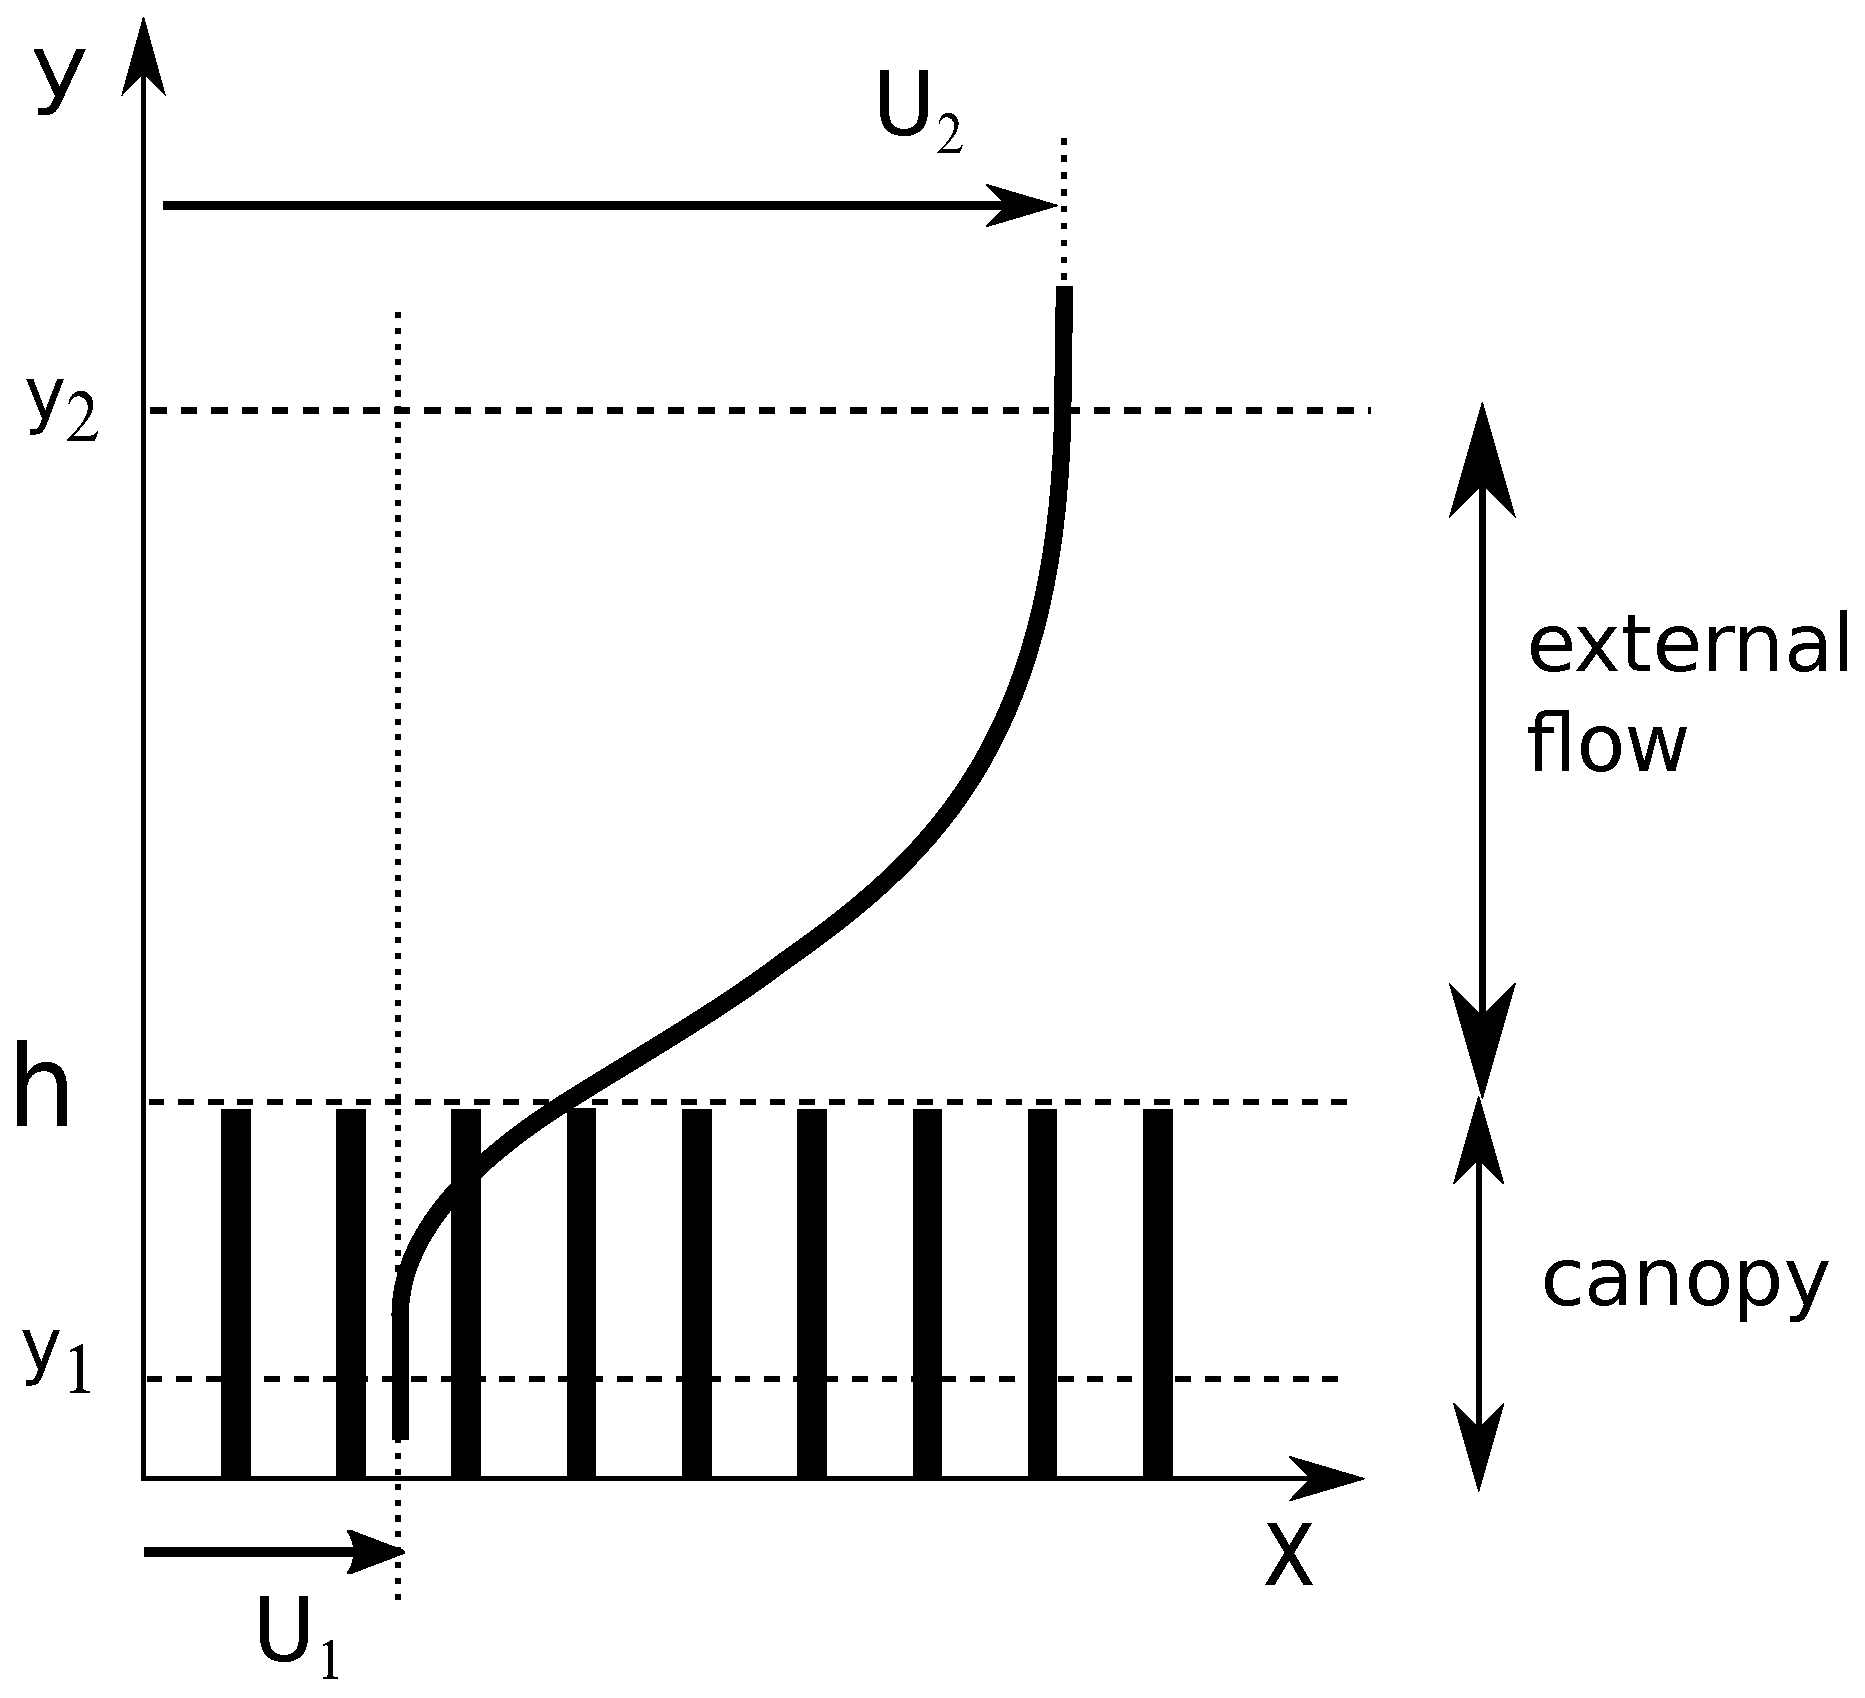
\includegraphics[width=0.5\linewidth]{chapter_3/figure/1}
	\caption{Configuration studied with main notations}
	\label{fig:1}
\end{figure}


\begin{figure}[h]
	\centering
	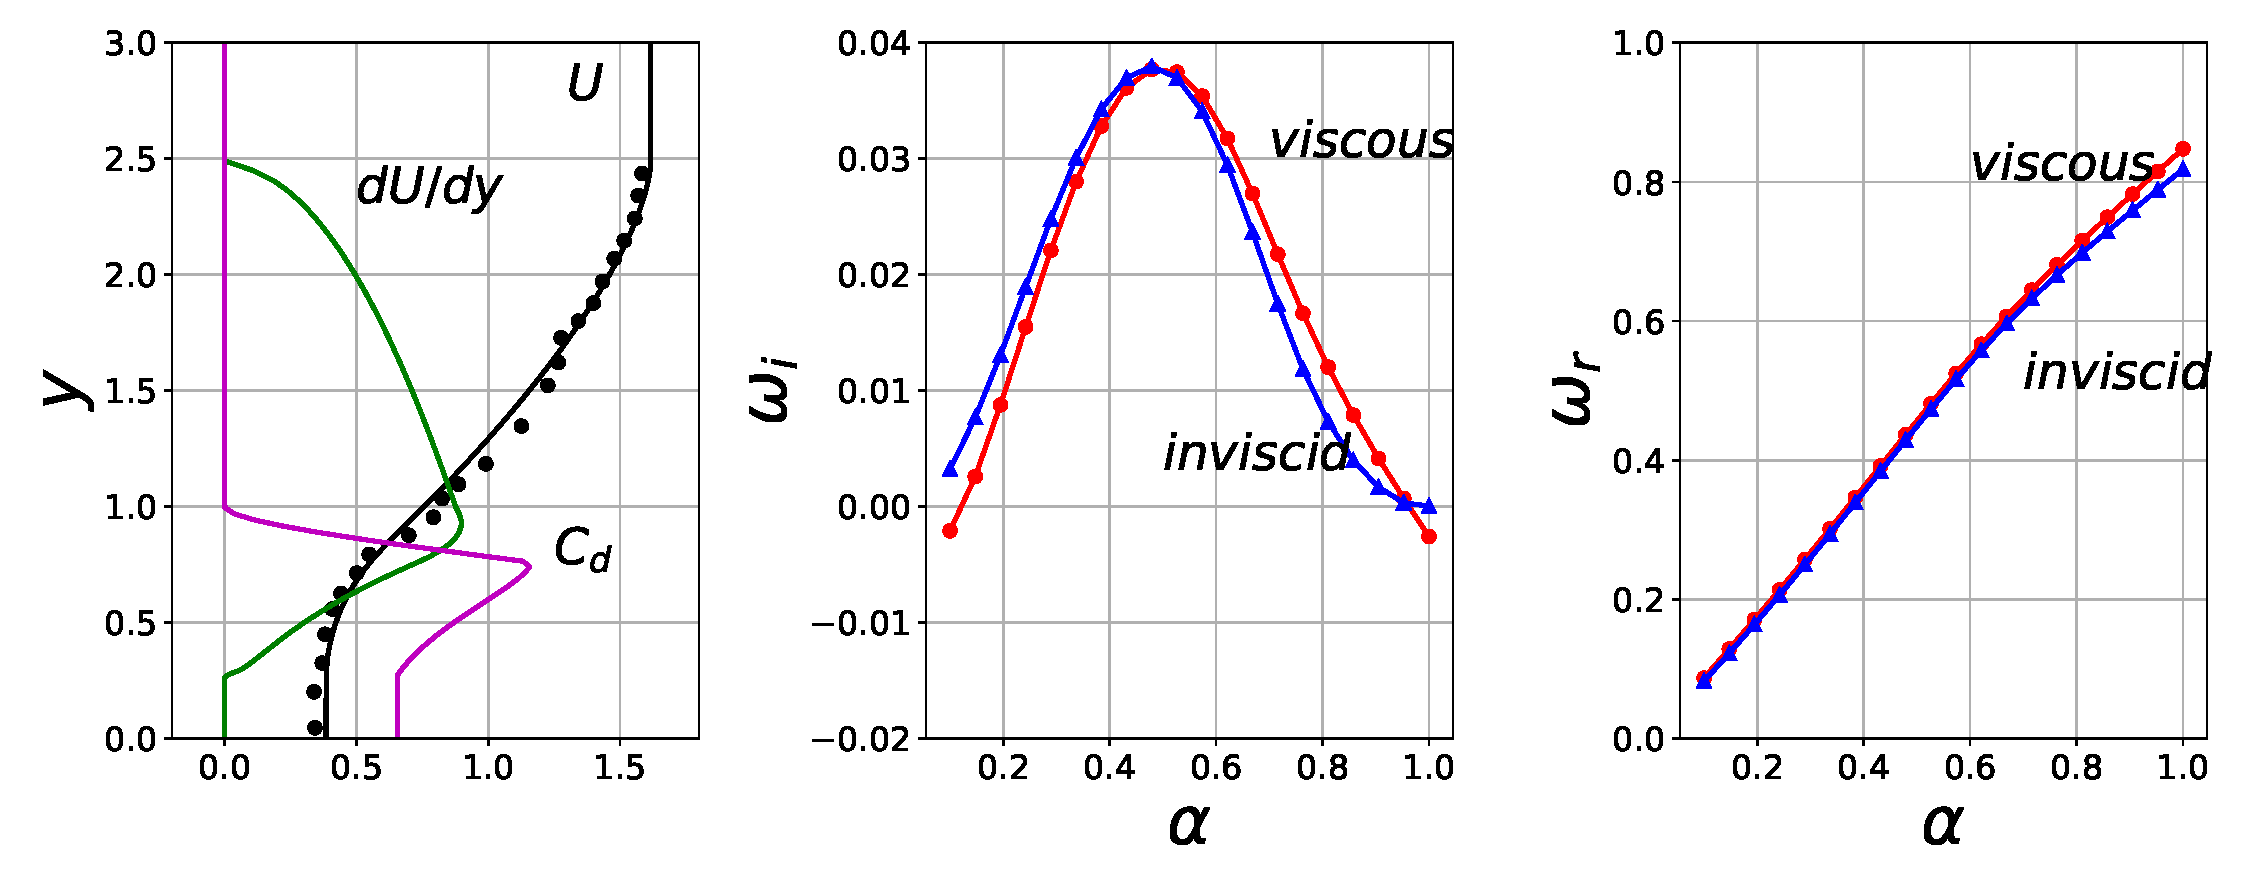
\includegraphics[width=1\linewidth]{chapter_3/figure/2}
	\caption{Left frame: mean flow U , together with experimental data points \citet{ghisalberti2004limited},  its first derivative, and drag coefficient
		distribution (case G). Center: viscous and inviscid growth rates, $\omega_i$ , as a function of the streamwise wavenumber $\alpha$. Right:
		corresponding frequencies, $\omega_r$}
	\label{fig:2}
\end{figure}



The Reynolds stress $\overline{u'v'}$ is modelled with
the Boussinesq assumption, introducing a turbulent viscosity which depends on a mixing length and
on the gradient of the mean velocity U. Referring to \citet{ghisalberti2004limited} for details of the empirical
correlations used to close the equations and the solution method, we limit ourselves here to stating
that the results obtained for the mean flow are very close to those reported in \citet{zampogna2016instability} (cf.
their Figure 3) and closely match experimental points for the cases G, H, I, and J considered (we use
the same terminology of\citet{ghisalberti2002mixing} \citet{ghisalberti2004limited} \citet{ghisalberti2005mass} to indicate the different flow configurations). An
example of mean flow is reported in \ref{fig:2} (left frame). There, one can observe the computed flow
(against discrete measurement points), its first derivative, and the drag coefficient distribution for one
representative case (experiment G), used below also to discuss stability and sensitivity results.
Other procedures have been employed in the past to calculate the mean flow, with satisfactory
results. For example,\citet{singh2016linear} have considered a constant value of $C_d$ through the canopy, while
\citet{zampogna2016instability} have coupled, at a fictitious interface, the fluid equations outside the canopy
to Darcy’s law within the vegetation. Thus, for the purposes of the present paper, the mean flow is
assumed as given; it could be, for example, simply a fit through experimental data. Nonetheless, in
Appendix A we provide some considerations on how $C_d$ affects the mean flow in the model used here.


%%%%%%%%%%%%%%%%%%%%%%%%%%%%%%%%%%%%%%%%%%%%%%%%%%%%%%%%%%%%%%%%%%%%%%
\subsection{Stability and sensitivity equations}
%%%%%%%%%%%%%%%%%%%%%%%%%%%%%%%%%%%%%%%%%%%%%%%%%%%%%%%%%%%%%%%%%%%%%%
\label{sec2b}
A temporal linear stability analysis is carried out, with the generic perturbation $q'(x, y,t)$ of the
form

\begin{equation}
q'(x,y,z,t)=\tilde q(y){\rm e}^{i(\alpha \  x -\omega \ t)}
\label{eq:q}
\end{equation}

with $\alpha$ the real streamwise wavenumber and $\omega$ a complex number whose real part, $\omega_r$ , is the fre-
quency of the mode and the imaginary part, $\omega_i$ , is the growth rate. The dimensionless linear stability
equations in primitive variables read

\begin{equation}
\begin{split}
& i\alpha u + D v =0,  \qquad D=d/dy \vspace{0.3cm}\\
& \left [ i (\alpha U -\omega)   - \frac{D^2-\alpha^2}{Re}+ a C_d U \right] u + U' v + i \alpha p  = 0,  \qquad U'=\dfrac{d U}{dy} \vspace{0.3cm} \\
& \left[ i (\alpha U -\omega)   - \frac{D^2-\alpha^2}{Re} \right ] v + D p   = 0
\label{eq:uvp}
\end{split}
\end{equation}

with the perturbation velocity components which vanish when $y=0$ and $y_{\infty}$. The upper boundary
of the computational domain is taken far enough away from the lower boundary to ensure that the
results do not vary upon modifications of $y_{\infty}$ . All the terms in the equations are dimensionless; the
mean speed through the shear layer, $U_m = \dfrac{U_1 +U_2}{2}$ , is used to scale the disturbance velocity components, pressure is scaled with
$\rho {U_m}^2$ , distances with $h$, and time with $h/U_m$ . The Reynolds number
in the equations above is thus defined as $Re = \rho U_m/ \mu h$ , with $\rho$ and $\mu$ the fluid’s density and dynamic
viscosity, respectively. The computations are performed both at the $Re$ values of the experiments
and in the inviscid limit (${Re}^{-1}  \rightarrow 0$ ), for comparison purposes. In the latter case, the boundary
conditions are simply $v = 0$ at $y = 0$ and $y_{\infty}$ .
System \ref{eq:uvp} above and its boundary conditions are, in the following, also written in short
notation as $\mathscr{L} q = 0$. The eigenvalues of the system are those complex values of $\omega$ which yield
non-trivial solutions for $u$, $v$, and $p$. Two numerical collocation codes are written, and success-
fully compared; one is based on the equations in primitive variables form, the second solves an
Orr-Sommerfeld-like equation (with the addition of the drag term) along the lines of \citet{singh2016linear}.
In both cases, a spectral scheme based on N Chebyshev polynomials is used (N is typically equal
to 300 to ensure grid-converged results), with an algebraic mapping between the physical and the
spectral domains (\citet{hussaini1987spectral} ).
Viscous and inviscid stability results for case G are shown in \ref{fig:2} (center and right frames);
differences are small, in consideration of the fact that the Reynolds number of the viscous case
is relatively large ($Re = 3450$). The viscous wavenumber of largest amplification is found for
$\alpha = 0.4790$; the waves are weakly dispersive, particularly at low wavenumbers (an original inter-
pretation of phase and group velocities is proposed in Appendix B). The wavelength of largest
growth is smaller than that found by \citet{zampogna2016instability} which was $0.73$; this is related to the slightly
different base flow in the two cases (in the present contribution a smoothing has been applied to the
$U$ velocity distribution to render $dU/dy$ continuous across $y$) and highlights the sensitivity of this
stability problem to base flow variations.
Following \citet{bottaro2003effect} it is assumed that small variations in base flow and drag coefficient
entail infinitesimal variations in the system’s eigenvalues and eigenfunctions. We stress here the fact
that $C_d$ is identically equal to zero outside of the canopy, and this implies that there are no possible
variations in $C_d$ for $y \geq 1$. The sensitivity functions to variations in $U$ and $C_d$ are obtained by using
the properties of the adjoint system which is defined from the Lagrange identity

\begin{equation}
0 = \delta \langle q^{\dagger}, \mathscr{L} q \rangle = 
\langle q^{\dagger}, \mathscr{L} \delta q \rangle +
\langle q^{\dagger}, \derp{\mathscr{L}}{U}  q \delta U\rangle +
\langle q^{\dagger}, \derp{\mathscr{L}}{C_d}  q \delta C_d\rangle +
\langle q^{\dagger}, \derp{\mathscr{L}}{\omega}  q \rangle \delta \omega
\label{eq:lagid}
\end{equation}

\begin{figure}[H]
	\centering
	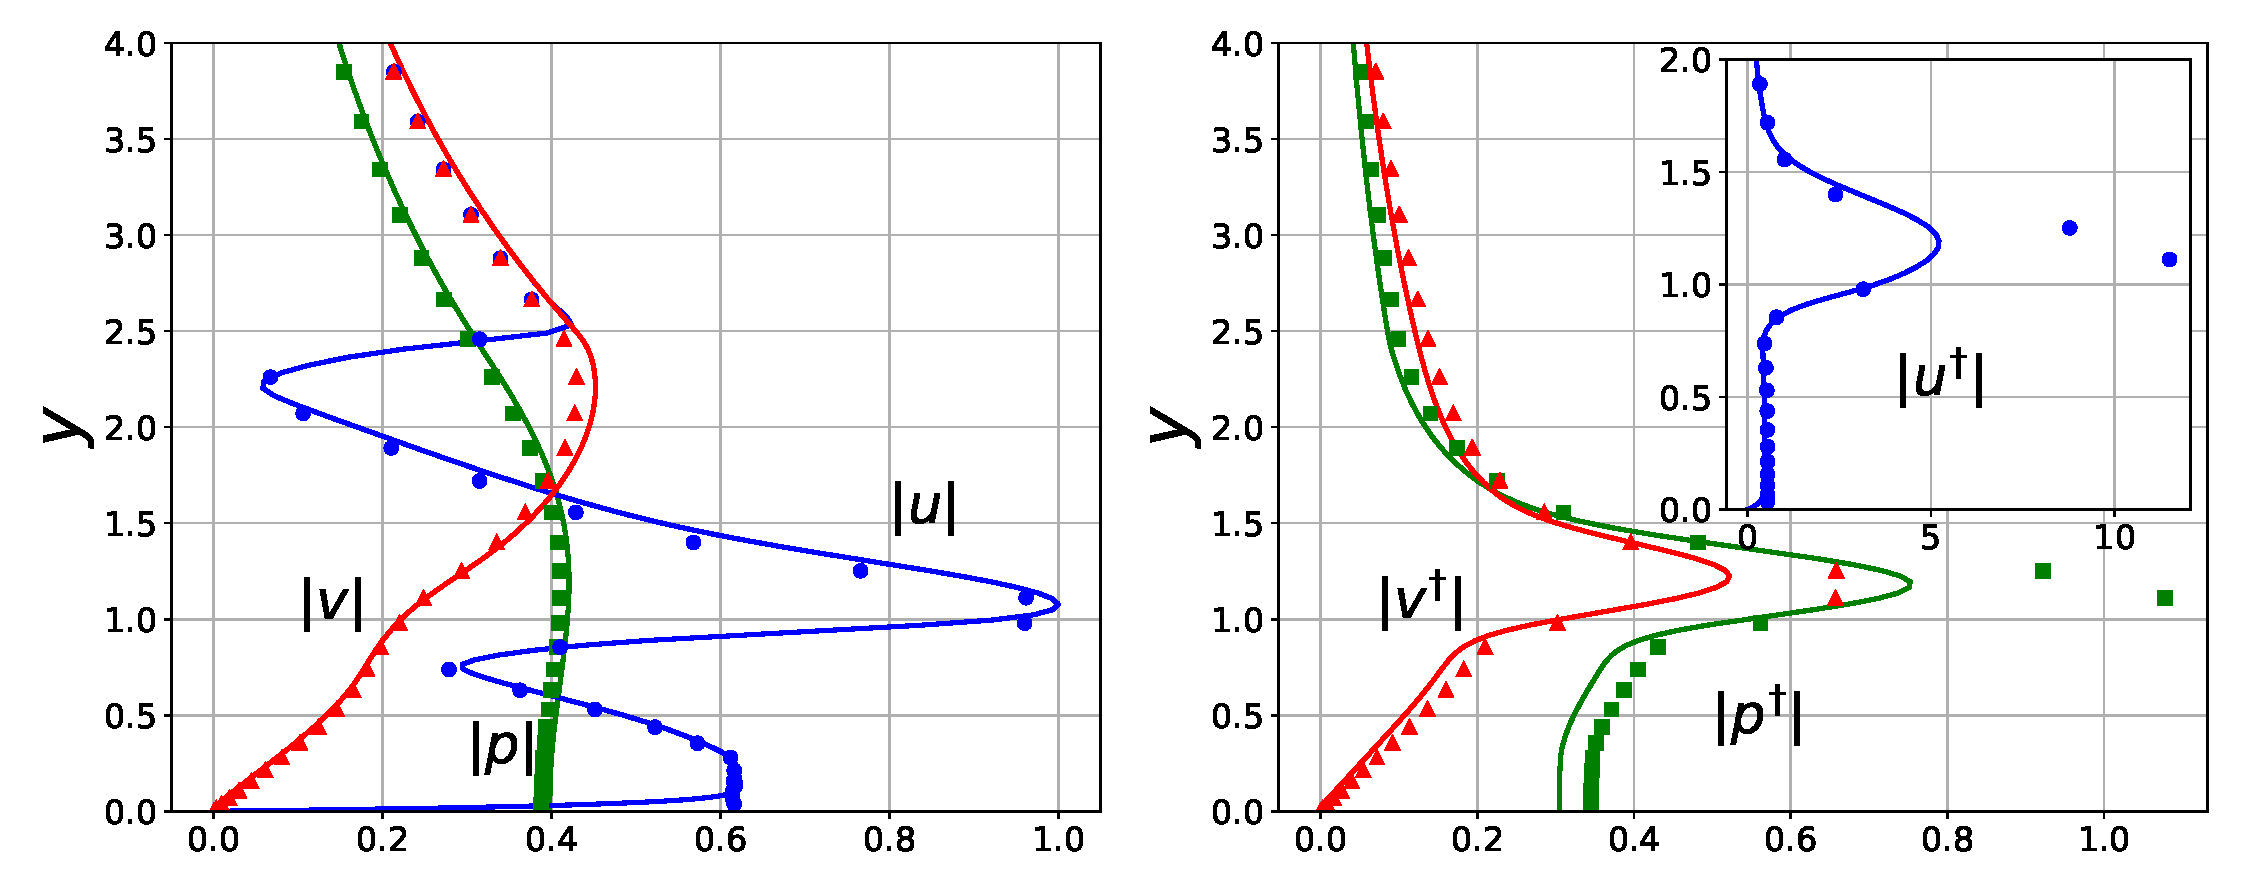
\includegraphics[width=1\linewidth]{chapter_3/figure/3}
	\caption{Moduli of direct (left frame) and adjoint (right frame) eigenfunctions for the viscous (continuous lines, $Re = 3450$)
		and the inviscid (symbols) case, in correspondence to the wavenumber of largest amplification.}
	\label{fig:3}
\end{figure}

and considering the effect of independent variations of $U$ and $C_d$ onto $q$ and $\omega$. It is found that

\begin{equation}
\delta \omega =\delta \omega_r + i \delta \omega_i= \int_0^{y_{\infty}}  G_U(y) \delta U(y) dy + \int_0^{1}  G_{C_D}(y) \delta C_D(y) dy
\label{eq:s_omega}
\end{equation}

with

\begin{equation}
\begin{split}
&G_{U} =  \alpha \left[ \overline{v^{\dagger}} v + \overline{u^{\dagger}} u  \right] +i   (\overline{u^{\dagger}}   v)' -i a C_d \overline{u^{\dagger}}  u \vspace{0.3cm}\\
&G_{C_D} =  - i \alpha  U  \overline{u^{\dagger}} u
\label{eq:GCD}
\end{split}
\end{equation}

the required sensitivity functions; the real parts of $G_U$ and $G_{C_d}$ express sensitivities to variations in
the frequency of the mode while the imaginary parts are sensitivities to variations in the growth rate.
Direct and adjoint eigenfunctions are normalized so that $N_{\omega} = 1$, with

\begin{equation}
N_{\omega} = \int_0^{y_{\infty}} \left[ \overline{ v^{\dagger}} v  +  \overline{ u^{\dagger}} u \right] dy
\label{eq:norm}
\end{equation}

An example of direct and adjoint eigenfunctions is provided in \ref{fig:3}, both in the viscous case
($Re = 3450$) and in the inviscid limit, for $\alpha = 0.4790$. It is interesting to observe that while the
direct eigenfunctions are almost overlapped, the same is not the case for the adjoint eigenfunctions,
with the inviscid mode (drawn with symbols) which has a larger amplitude than the viscous one.
The shapes of the direct eigenfunctions are very close to those reported in \citet{zampogna2016instability}. The adjoint modes
reveal that the flow is most sensitive to streamwise forcing, particularly when it occurs slightly
above the edge of the canopy. Source terms in the mass conservation and in the vertical momentum
equations are much less effective.


%%%%%%%%%%%%%%%%%%%%%%%%%%%%%%%%%%%%%%%%%%%%%%%%%%%%%%%%%%%%%%%%%%%%%%
\section{Sensitivity results for the isotropic drag model}
%%%%%%%%%%%%%%%%%%%%%%%%%%%%%%%%%%%%%%%%%%%%%%%%%%%%%%%%%%%%%%%%%%%%%%
\label{sec:3}

Some representative sensitivity functions are plotted in \ref{fig:4}; viscous and inviscid results
concur in showing that the largest sensitivities to variations of U are found right above the vegeta-
tion’s edge, where there are peaks in the adjoint eigenfunctions and where $d^2 U/d y^2$ vanishes. The
$U$-sensitivities are negligible within the vegetated layer and for values of $y$ larger than twice the
canopy’s height. The $C_d$-sensitivities are non-negligible only in close proximity of the interface.
It is interesting to observe that real and imaginary parts of the $U$-sensitivity functions are
shifted in y with respect to one another; this means that, for example, a localized perturbation at
a given $y$ position (above the canopy) might have a strong repercussion on the growth rate but not
on the frequency of the most unstable Kelvin-Helmholtz mode, or vice versa. Comparing left and
right frames of the figure, it is seen that inviscid $G_U$ sensitivity functions display sharper peaks and
steeper gradients, and yield larger variations in $\omega$ than their viscous counterparts in the proximity of
the $U$ inflection point, a clear consequence of the inviscid mechanism ruling the instability. In both
the viscous and the inviscid models, the sensitivity to base flow variations is typically one order of
magnitude larger than the sensitivity to changes in the drag coefficient.

\begin{figure}[H]
	\centering
	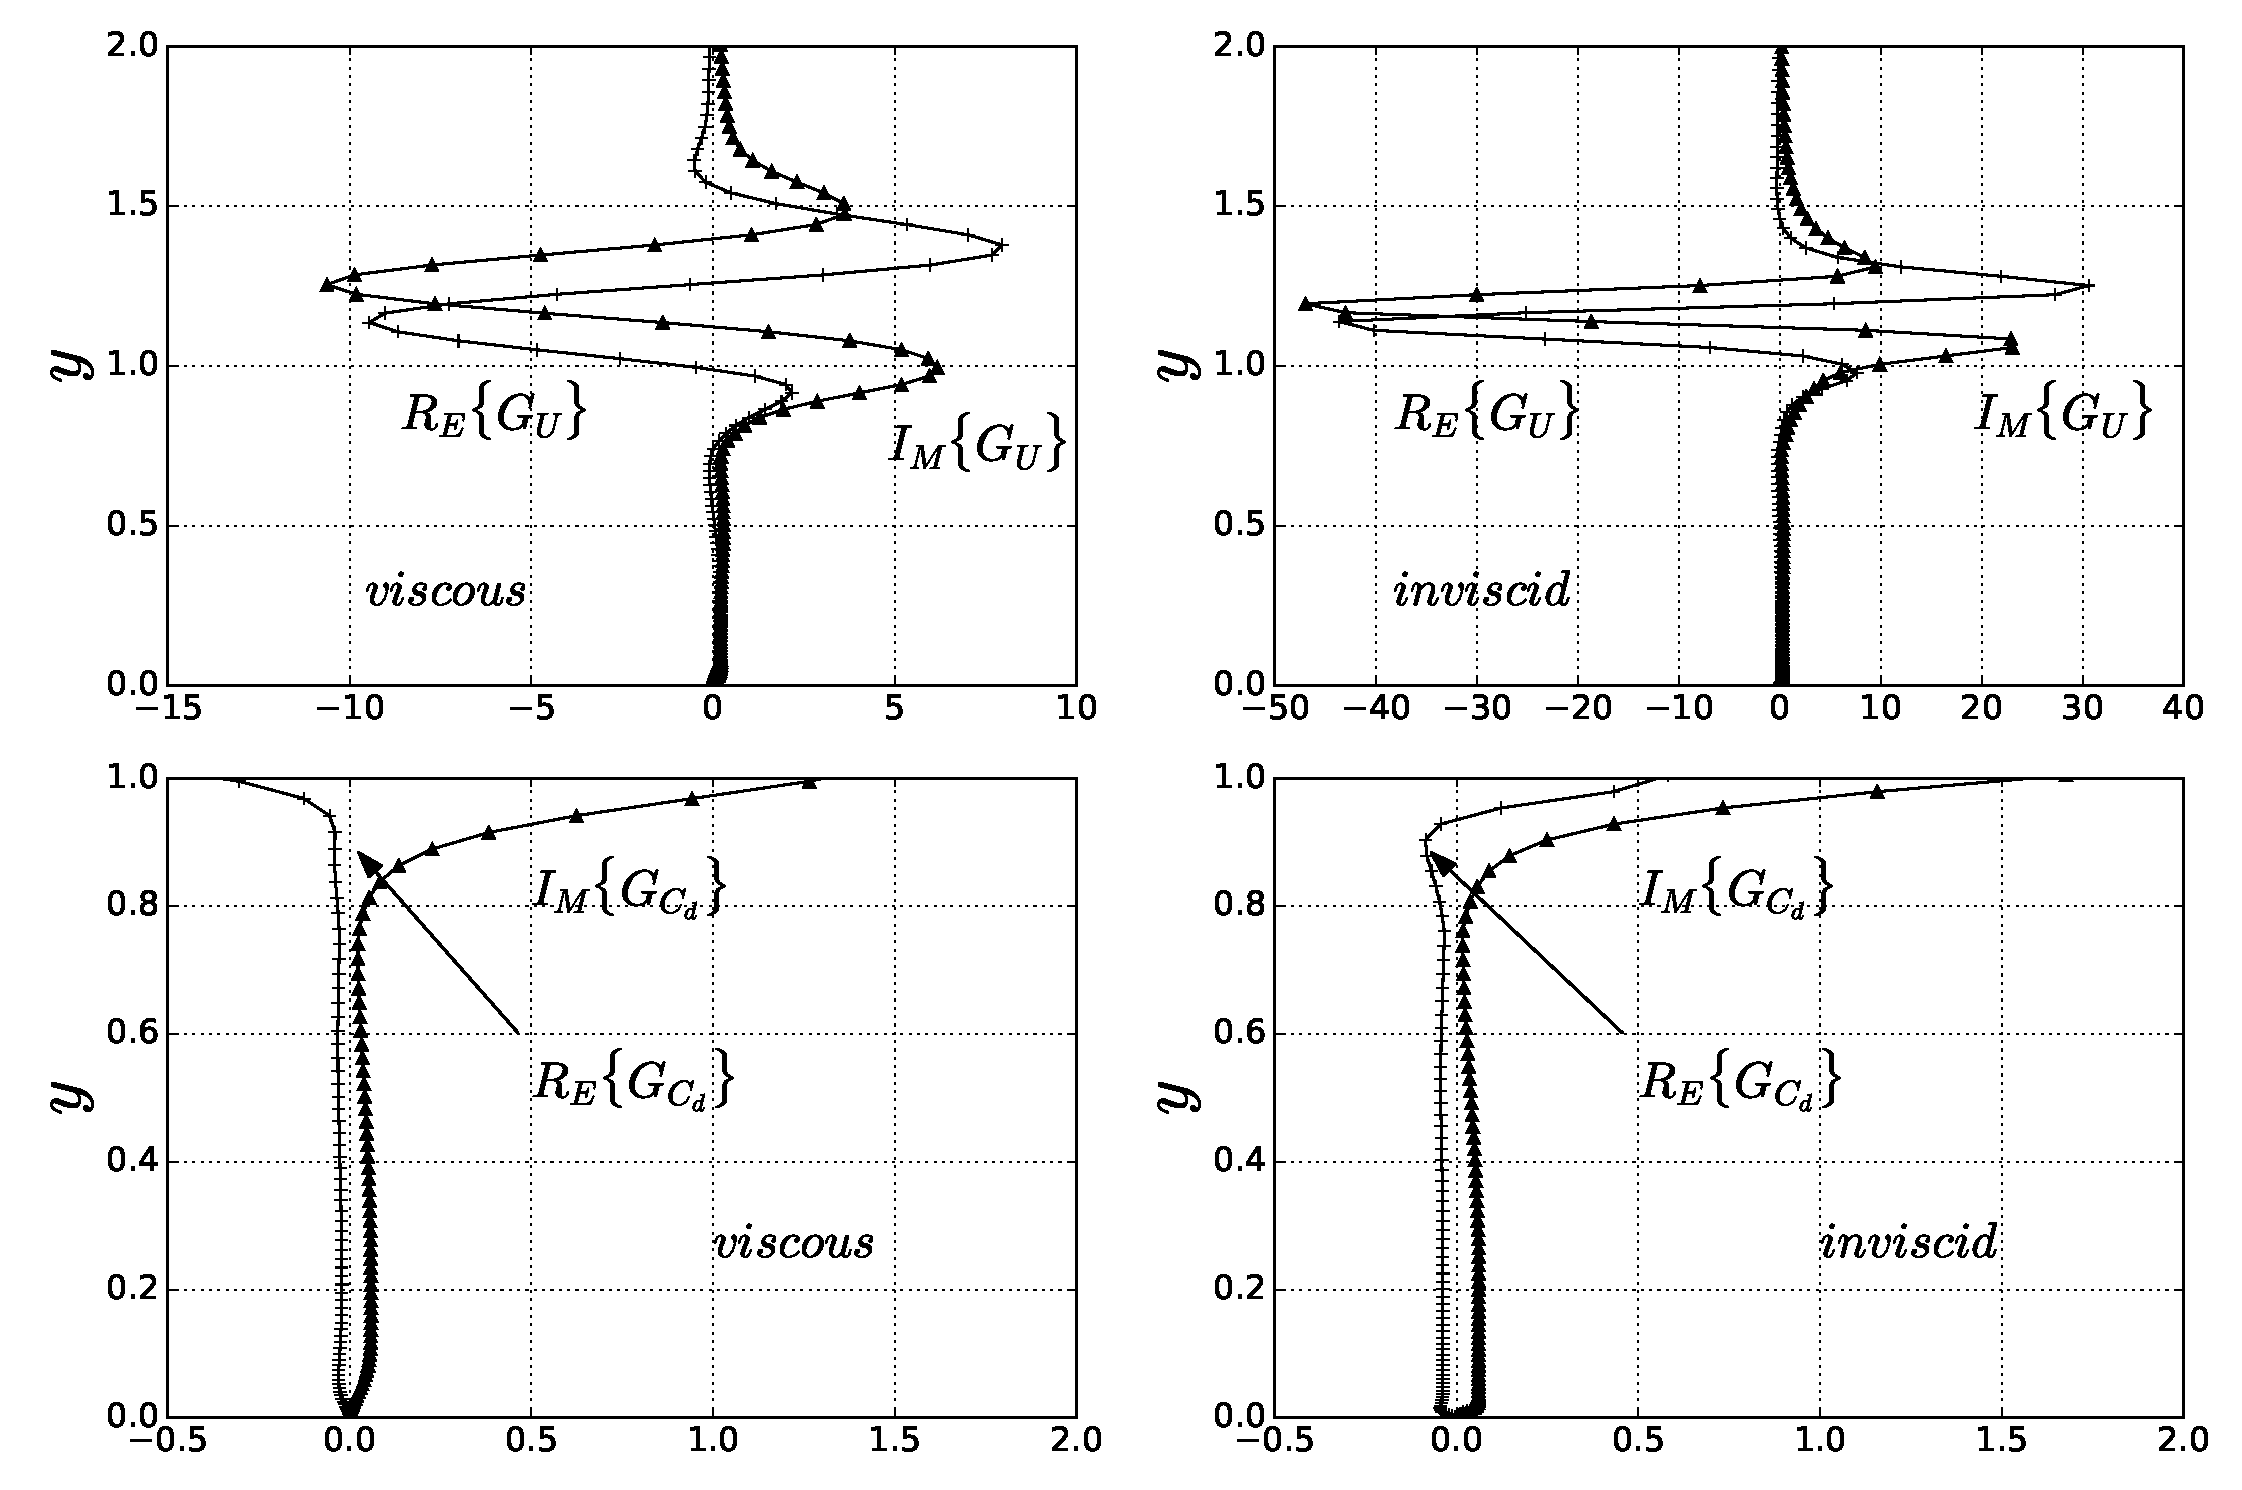
\includegraphics[width=1\linewidth]{chapter_3/figure/4}
	\caption{Real and imaginary parts of the sensitivities to mean flow variations (top) and to variations in the drag distribution
		function (bottom), for the parameters of \ref{fig:3}}
	\label{fig:4}
\end{figure}

The infinite norm of the sensitivities for the four cases studied (G, H, I, and J) is reported in
\ref{fig:5}; the main result found is that ${|G_U|}_{\infty}$ grows monotonically with $\alpha$ (and more so in the inviscid
case) whereas ${|G_{C_d}|}_{\infty}$ does not. It is consistently found that ${|G_U|}_{\infty}$ of case H is larger than that of
case I, which exceeds the corresponding value of case J, in turn larger than${|G_U|}_{\infty}$ of case G. This is
not unexpected in view of the values of the mean shear $\dfrac{U_2 - U_1}{H}$  which are, going from H to G, equal

\begin{figure}[H]
	\centering
	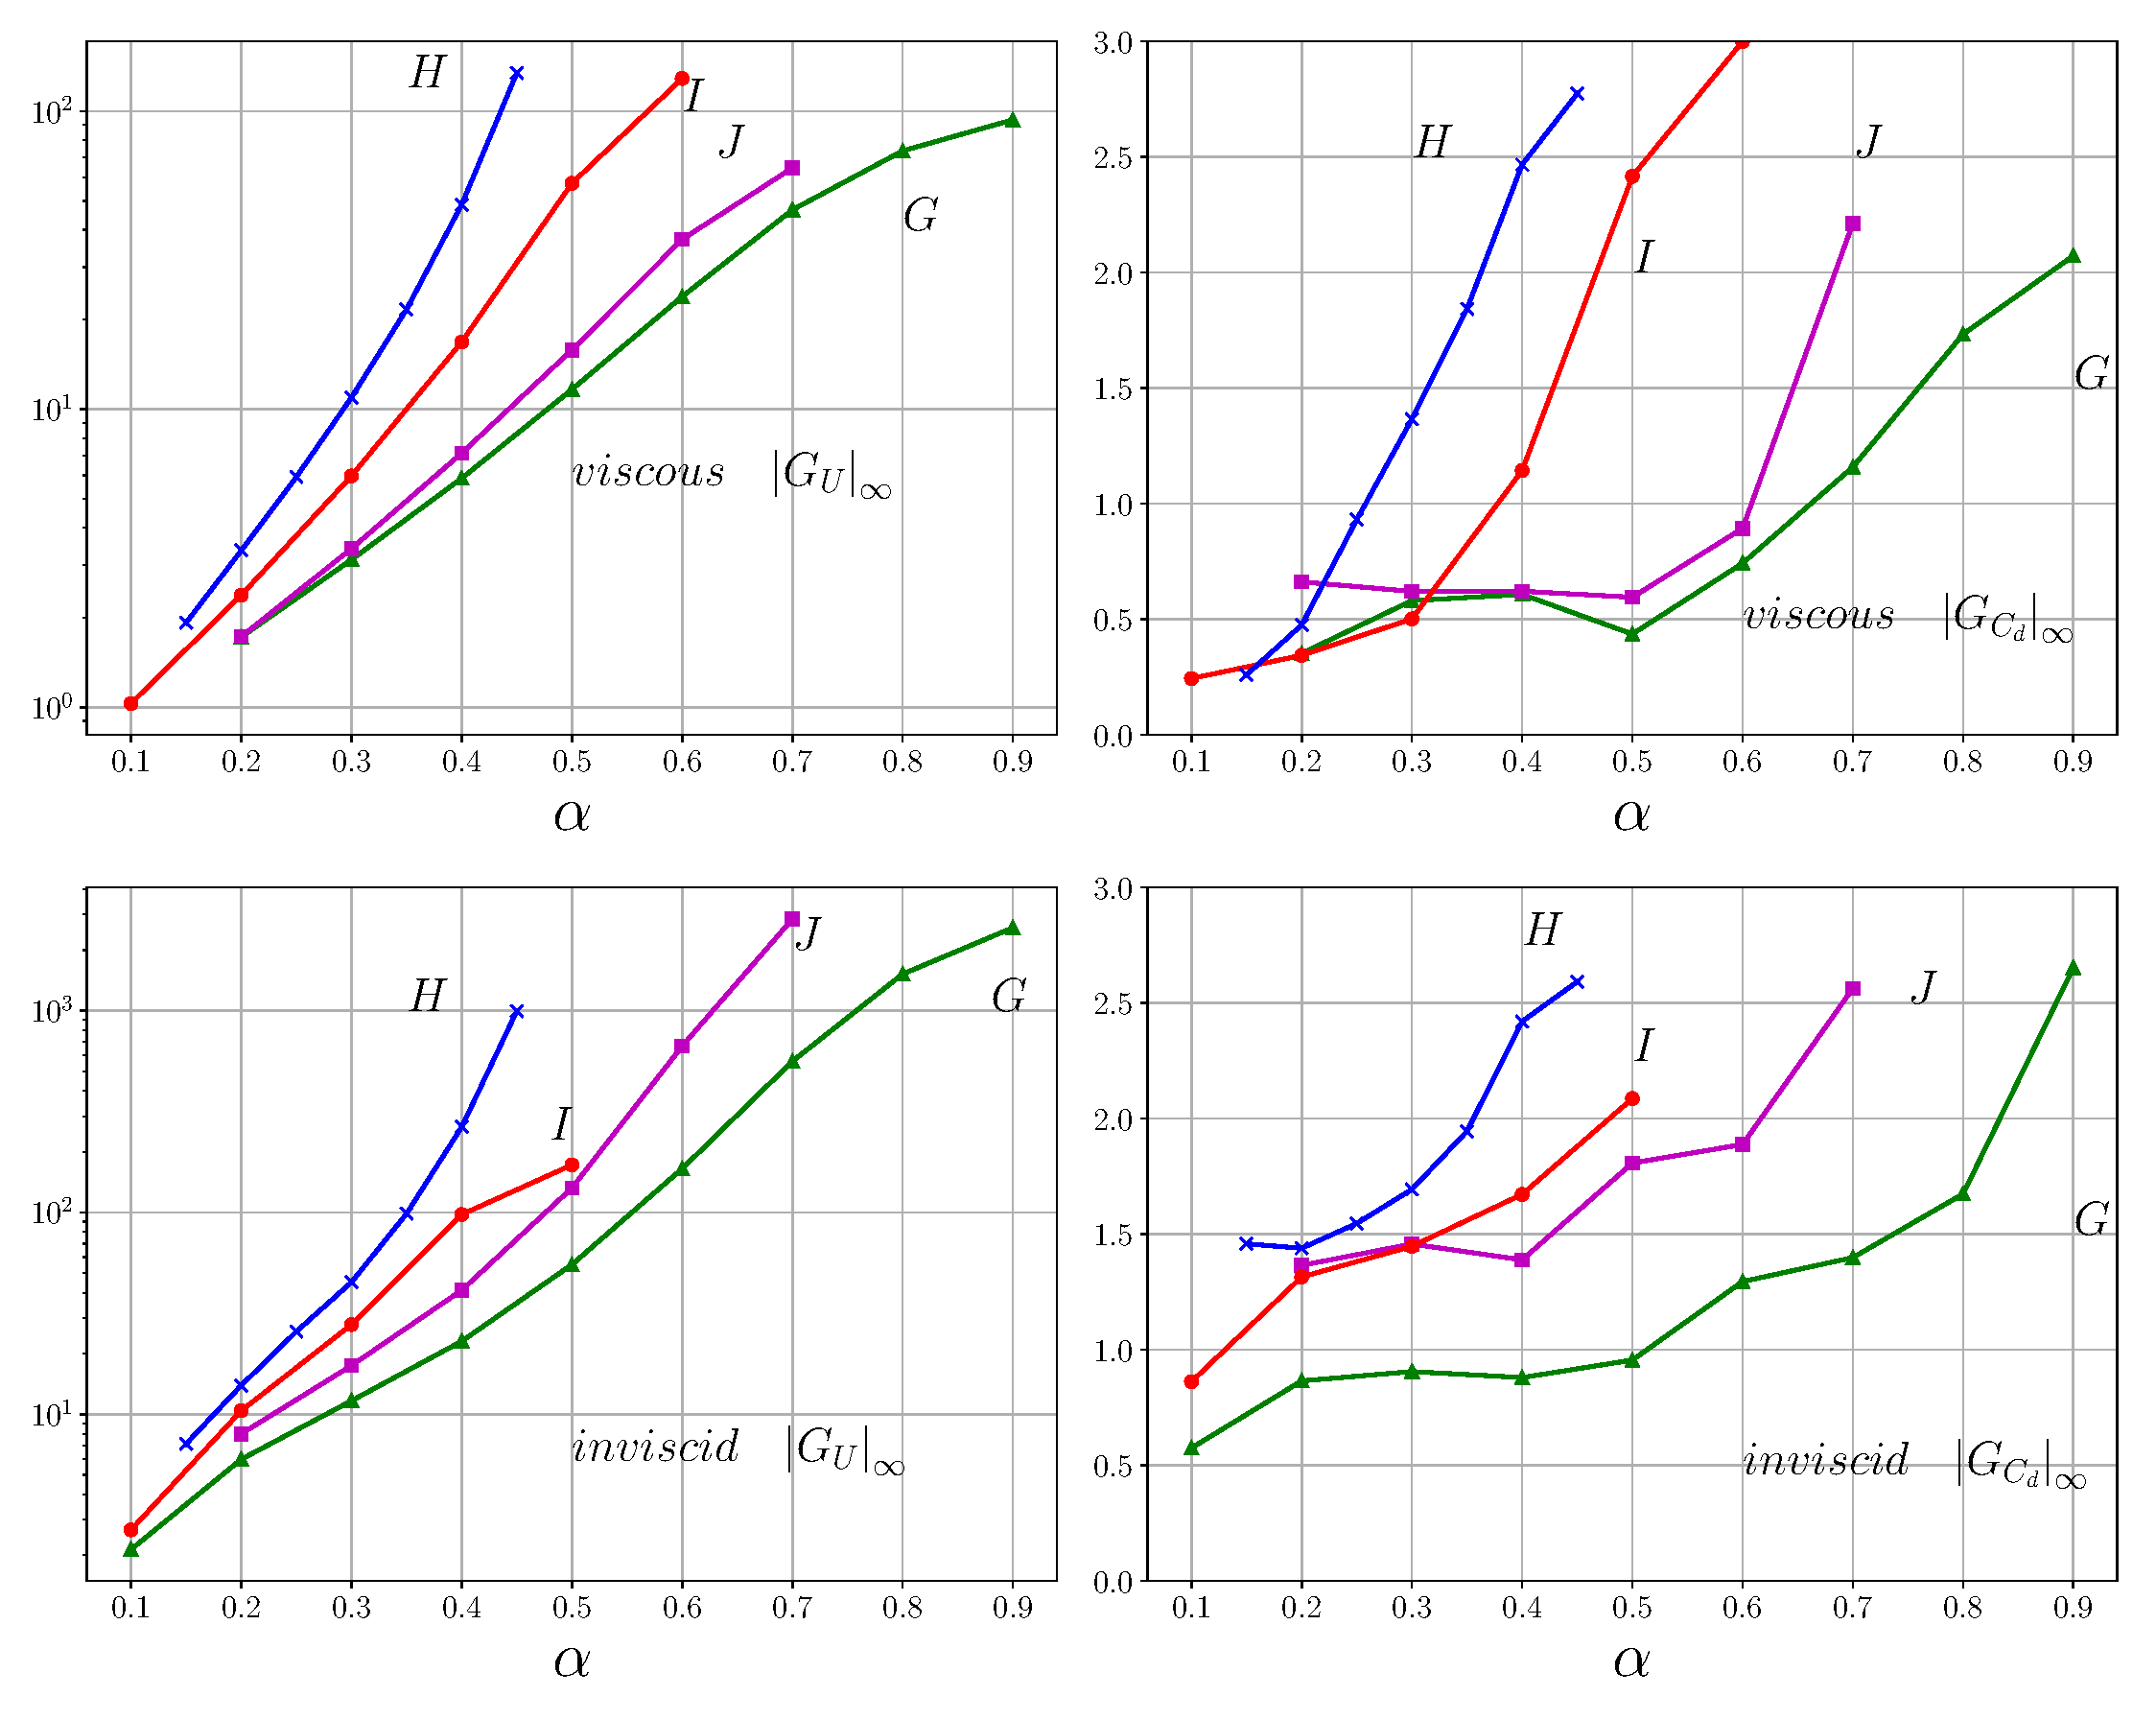
\includegraphics[width=1\linewidth]{chapter_3/figure/5}
	\caption{Infinite norms of the sensitivity functions for varying $\alpha$}
	\label{fig:5}
\end{figure}

to $0.236$, $0.158$, $0.084$, and $0.071 s^{-1}$ , respectively. The sensitivity of the eigenvalue $\omega$ to variations
in the mean flow is generally stronger than the corresponding sensitivity to variations in the drag
coefficient (aside for the long wave limit, where they are comparable). This might be interpreted
positively, considering that the use of a scalar coefficient $C_d$ to represent the drag within the canopy
is but a crude approximation. An alternative model to represent the flow throughout a network of
rigid, cylindrical dowels has recently been proposed by \citet{zampogna2016instability} The sensitivity results for
such a new model are discussed next.


%%%%%%%%%%%%%%%%%%%%%%%%%%%%%%%%%%%%%%%%%%%%%%%%%%%%%%%%%%%%%%%%%%%%%%
\section{An alternative sensitivity model: accounting for the canopy anisotropicity}
%%%%%%%%%%%%%%%%%%%%%%%%%%%%%%%%%%%%%%%%%%%%%%%%%%%%%%%%%%%%%%%%%%%%%%
\label{sec:4}

The stability problem in this section is based on the coupling between two regions, one outer
region dominated by inertia and ruled by the inviscid equations and an inner one dominated by
viscosity and ruled by Darcy’s law, with account of the canopy geometry through a tensorial
permeability, as described by \citet{zampogna2016instability} Normalizing the disturbance equation which couples
pressure and velocity in the inner region with the same scales as previously, we obtain

\begin{equation}
{u_i}' = -Re \dfrac{d}{ah^2} \mathcal{K}_{ij} \derp{p'}{{}x_j}',  \qquad (x_1, x_2) = (x,y)
\label{eq:darcy}
\end{equation}


with $\mathcal{K}_{ij}$ the dimensionless permeability. The effective interface between the inertial region and the
slow, viscosity-dominated region does not coincide with the edge of the canopy; in fact, the rapid
outer flow penetrates through the upper part of the vegetation and an effective matching between
outer and inner flows must be enforced some distance $\delta$ below the canopy’s edge \citet{le2006interfacial}.  This distance,
a penetration depth, has been successfully computed by \citet{zampogna2016fluid} for a few cases
and is found to increase with the Reynolds number of the flow; for experiment G discussed below it
is$ \delta = 0.40$ \citet{zampognaprivate}. On account of the results shown in \ref{fig:4}, with the sensitivities which are negligible
for $y \approx 0.60$, we expect that the exact position of the effective interface will not affect the results
significantly.
Using the fact that the velocity within the orthotropic porous medium is divergence free, the
interface condition to be applied at $y_{itf} = 1 - \delta$ is found to be \ref{eq:darcybc}

\begin{equation}
v|_{itf} + B(\alpha) p|_{itf} = 0
\label{eq:darcybc}
\end{equation}

with

$$
B(\alpha) = Re \dfrac{d}{ah^2} \sqrt{\mathcal{K}_{11}\mathcal{K}_{22}} \alpha \tanh (\theta), \qquad \theta = \alpha \sqrt{\dfrac{\mathcal{K}_{11}}{\mathcal{K}_{22}}}  y_{itf}
$$

The second boundary condition that the Rayleigh stability equation must satisfy at $y_{\infty}$ is sim-
ply $v = 0$. Thus, we solve only for the inviscid flow in the outer region, and the permeability
of the inner domain enters the equations only through the interface condition \ref{eq:darcybc}. $\mathcal{K}_{ij}$ is a two-
by-two diagonal tensor; $\mathcal{K}_{11}$ is the component of the dimensionless permeability along $x$ and
$\mathcal{K}_{22}$ is the $y$ component. For case G considered here, the packing density of the elements is
$a = 0.04 cm^{-1}$ ; it is also found that $\mathcal{K}_{11}= 0.0512$ and $\mathcal{K}_{22} = 0.0575$ \citet{zampognaprivate},  so that the function $B(\alpha)$
reads $B = 15.727 \alpha \tanh (0.566 \alpha)$.


%%%%%%%%%%%%%%%%%%%%%%%%%%%%%%%%%%%%%%%%%%%%%%%%%%%%%%%%%%%%%%%%%%%%%%
\subsection{The sensitivity equations}
%%%%%%%%%%%%%%%%%%%%%%%%%%%%%%%%%%%%%%%%%%%%%%%%%%%%%%%%%%%%%%%%%%%%%%

The adjoint equations in this case are the same as system \ref{eq:uvp}, without the terms containing $1/Re$
and $C_d$ , and the boundary conditions are

\begin{equation}
v^{\dagger}|_{itf} - B(\alpha) p^{\dagger}|_{itf} = 0, \qquad v^{\dagger}|_{y_{\infty}} = 0
\label{eq:darcybc_adjoint}
\end{equation}

The variation in the complex frequency is related to variations in the mean flow and in the perme-
ability components through the equation

$$
\delta \omega = \int_{y_{itf}}^{y_{\infty}}  G_U(y) \delta U(y) dy + G_{\mathcal{K}_{11}} \delta \mathcal{K}_{11} + G_{\mathcal{K}_{22}} \delta \mathcal{K}_{22}
$$

\begin{figure}[H]
	\centering
	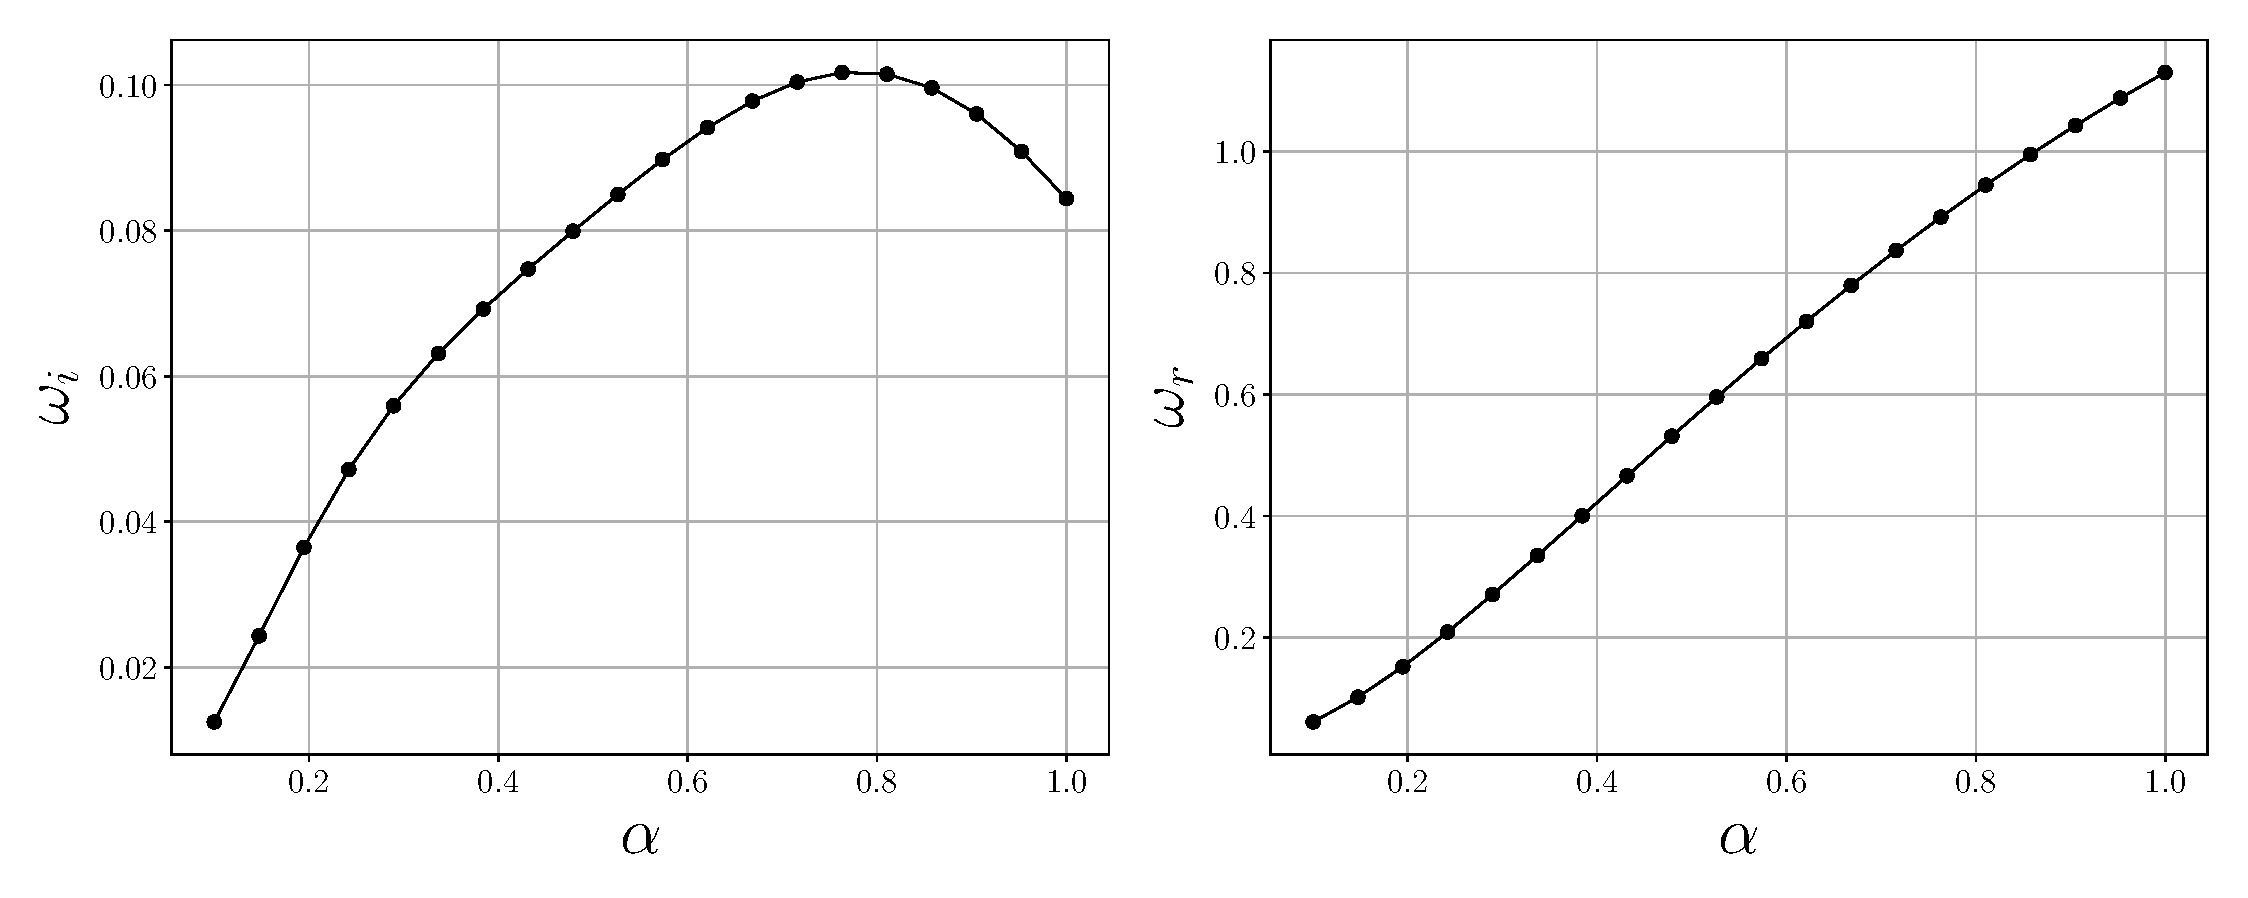
\includegraphics[width=1\linewidth]{chapter_3/figure/6}
	\caption{Amplification factor (left) and frequency of the most unstable mode as a function of $\alpha$, for the anisotropic drag
		model}
	\label{fig:6}
\end{figure}


with

\begin{equation}
\begin{split}
& G_U = \alpha  \left[  \overline{v^{\dagger}} v +  \overline{u^{\dagger}} u \right] + i ( \overline{u^{\dagger}} v)'  \vspace{0.3cm}\\
& G_{\mathcal{K}_{11}} = -\dfrac{i}{2} \alpha Re \dfrac{d}{a h^2}  \left[  \overline{p^{\dagger}} p \right]|_{itf} \sqrt{\dfrac{\mathcal{K}_{22}}{\mathcal{K}_{11}}} \left\lbrace \tanh \theta + \dfrac{\theta}{\cosh^2 \theta}\right\rbrace	\vspace{0.3cm}\\
& G_{\mathcal{K}_{22}} = -\dfrac{i}{2} \alpha Re \dfrac{d}{a h^2}  \left[  \overline{p^{\dagger}} p \right]|_{itf} \sqrt{\dfrac{\mathcal{K}_{11}}{\mathcal{K}_{22}}} \left\lbrace \tanh \theta - \dfrac{\theta}{\cosh^2 \theta}\right\rbrace
\end{split}
\end{equation}


the required sensitivities, with the normalization  $\int_{y_{itf}}^{y_{\infty}} \left[  \overline{v^{\dagger}} v +  \overline{u^{\dagger}} u \right] = 1$.
In writing $\delta \omega$ above, we have made the assumption that the mean flow $U$ does not vary at the two extreme points of the
integration domain.
The stability results (for the same parameters as in \ref{fig:2}) are displayed in \ref{fig:6}. As already
observed in \citet{zampogna2016instability}, both the growth rate and the frequency are slightly larger with this model than
with the isotropic resistance model, for all $\alpha$’s, and the most unstable mode is found at a larger
value of $\alpha$ (here $\alpha \approx 0.8$) in better agreement with experimental correlations \citet{zampogna2016instability} \citet{raupach1996coherent}.  Also in this case the
waves are found to be only weakly dispersive.
Eigenfunctions are plotted in \ref{fig:7}, together with the real and imaginary parts of the $G_U$
sensitivity function. As in \ref{fig:3}, the modulus of the $u$ eigenfunction peaks near the edge of the
canopy ( $y = 1$), whereas the adjoint eigenfunctions have a maximum value slightly above. As a
general remark, the shapes of the direct and adjoint modes are quite similar to those found with
the isotropic resistance model; as reported at the end of \ref{sec2b}, it is found that the flow
is most sensitive to streamwise momentum forcing. Also, real and imaginary parts of $G_U$ have a
double-peak structure, like in the isotropic-drag model, but now the largest absolute value of $G_U$ is

\begin{figure}[H]
	\centering
	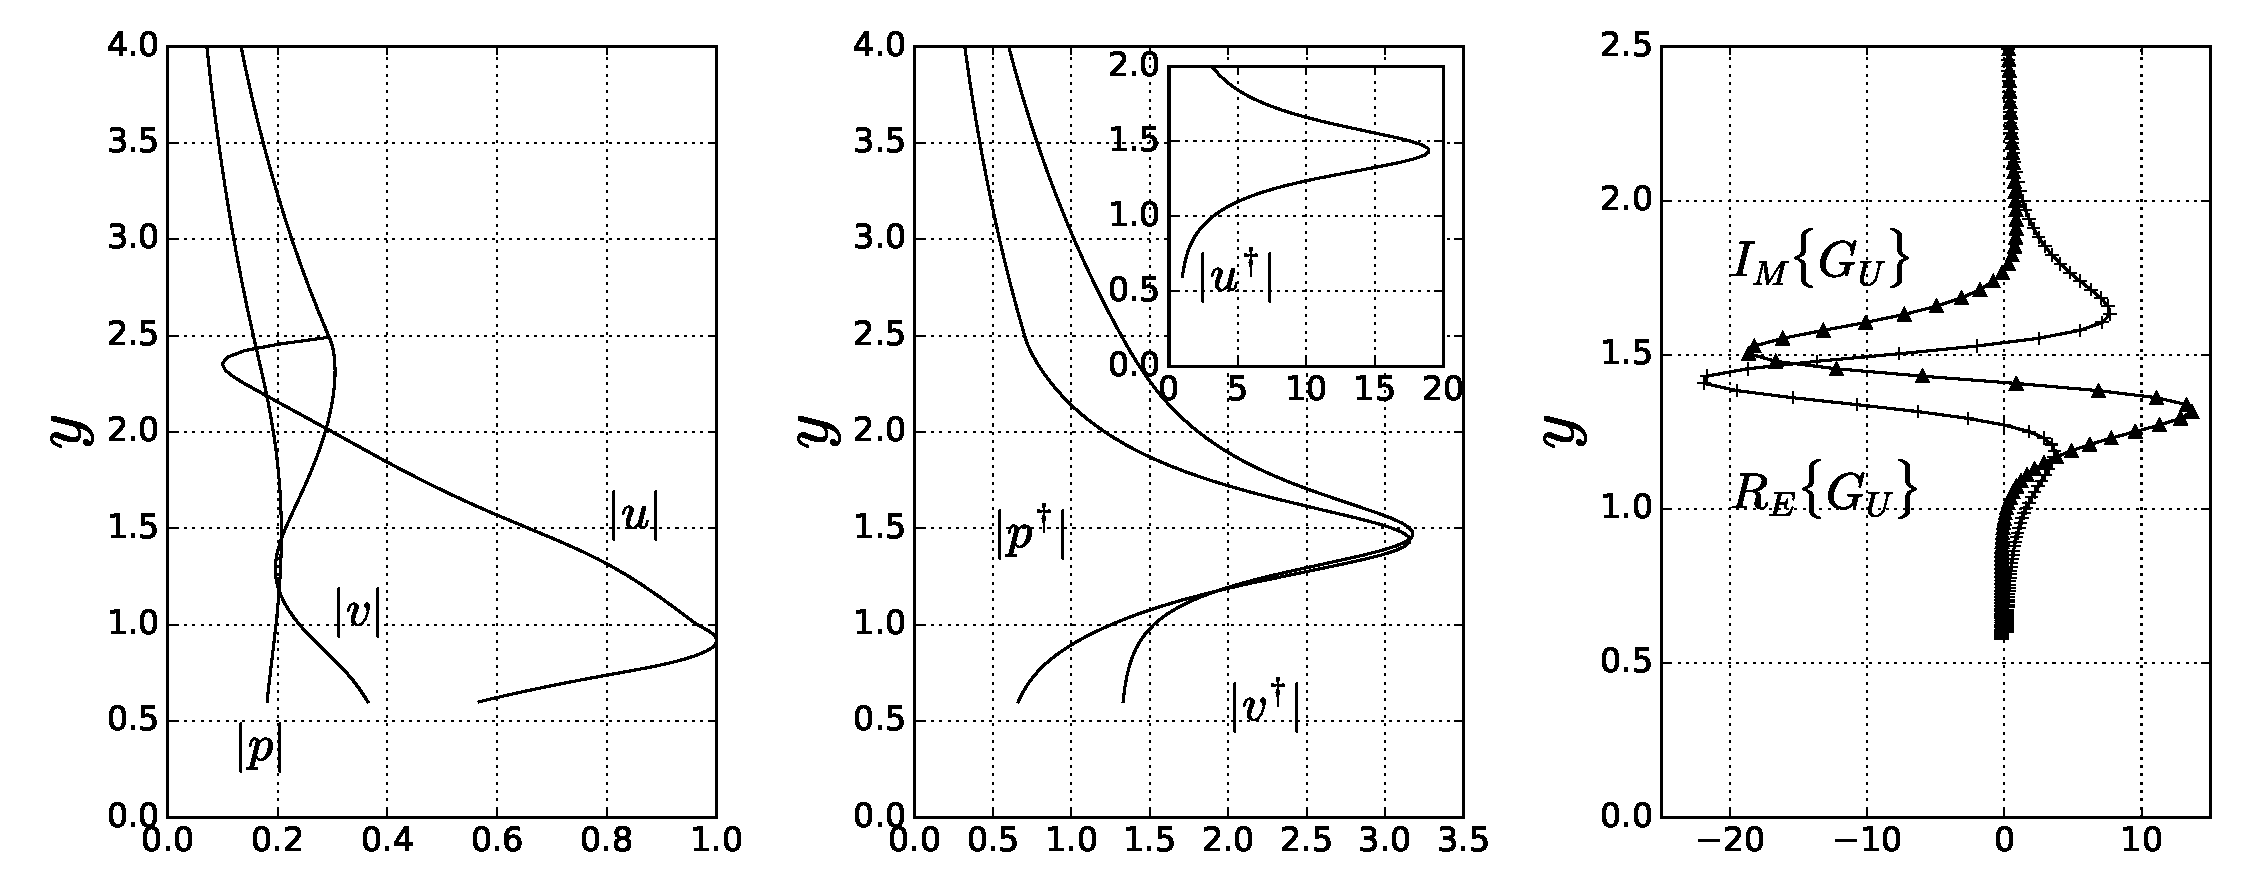
\includegraphics[width=1\linewidth]{chapter_3/figure/7}
	\caption{Left and center frames: moduli of direct and adjoint eigenfunctions; pressure and “adjoint pressure” are drawn with
		dashed lines. Right: real and imaginary parts of the sensitivity function $G_U$ ($\alpha = 0.4790$)}
	\label{fig:7}
\end{figure}

\begin{figure}[H]
	\centering
	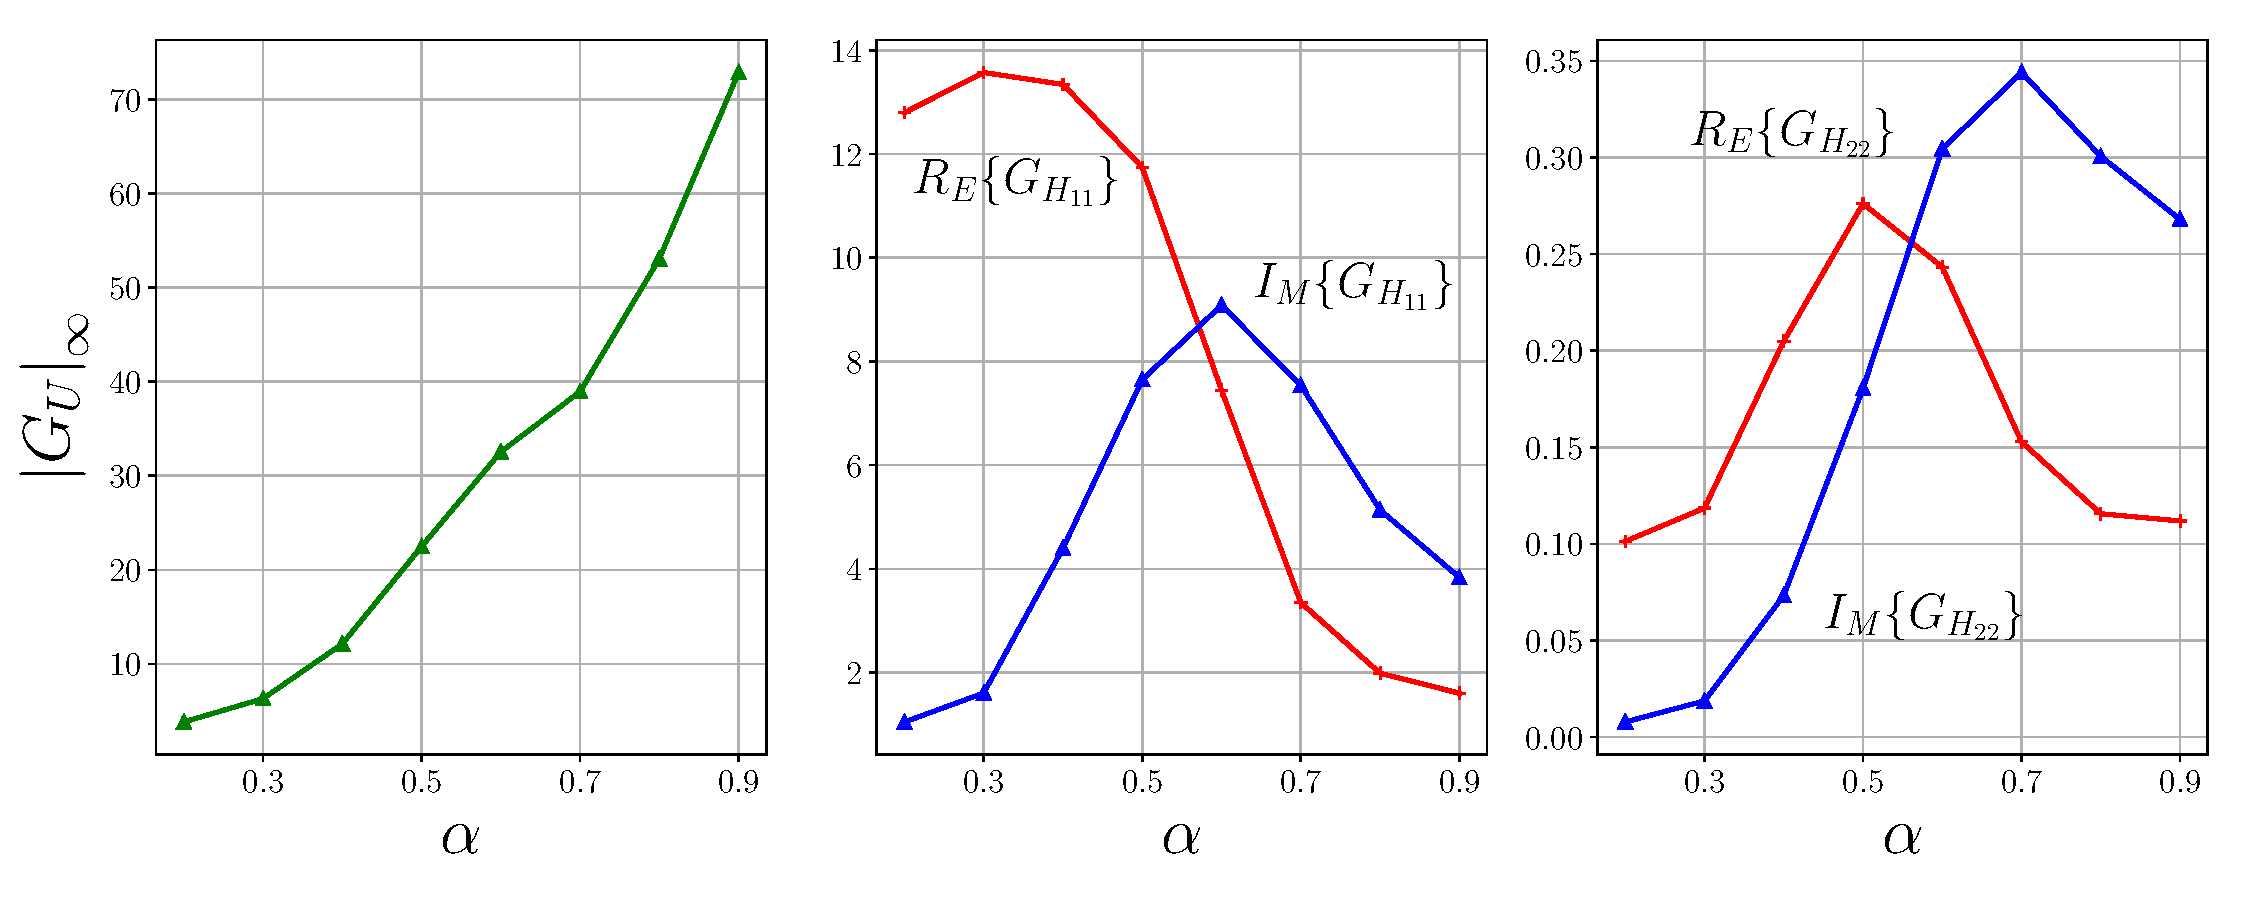
\includegraphics[width=1\linewidth]{chapter_3/figure/8}
	\caption{Case G. Left: infinite norm of $G_U$ for varying $\alpha$. Center and right frames: real and imaginary parts of the sensitivity
		coefficients to variations in the permeability components}
	\label{fig:8}
\end{figure}

smaller and shifted towards a larger y than in the previous inviscid case (cf.\ref{fig:4}, top-right frame).
This can also be appreciated by the inspection of \ref{fig:8} (left); $|G U |_{\infty}$ still grows monotonically with
$\alpha$, but the sensitivity is smaller than that computed earlier (cf. \ref{fig:5}) with either the viscous or
inviscid model (it is actually closer to the viscous sensitivity, as an effect of the interface condition).
Furthermore, it is interesting to observe that both real and imaginary parts of $G_U$ vanish for $y = y|_{itf}$
(cf.\ref{fig:7}, right), and this supports the statement made previously that a small shift in the position
of the effective interface has but a minor influence on the most unstable mode.
The sensitivity coefficients for the two components of the permeability tensors are displayed in
\ref{fig:8} (center and right frames): the present model is more effective to variations in $\mathcal{K}_{11}$ than to $\mathcal{K}_{22}$
as far as modifying the complex eigenfrequency. Significantly, different ranges of wavenumbers
behave differently as far as the variation in $\omega$ is concerned. The frequency $\omega_r$ of long waves (around
$\alpha \approx 0.3$) is more easily modified by acting on $\mathcal{K}_{11}$ (with an almost negligible effect on the growth
rate of the wave); conversely, the growth rate of modes with large values of $\alpha$ is affected efficiently
by variations in the first component of the permeability tensor.

%%%%%%%%%%%%%%%%%%%%%%%%%%%%%%%%%%%%%%%%%%%%%%%%%%%%%%%%%%%%%%%%%%%%%%
\section{Concluding remarks}
%%%%%%%%%%%%%%%%%%%%%%%%%%%%%%%%%%%%%%%%%%%%%%%%%%%%%%%%%%%%%%%%%%%%%%
We have considered two different models of the flow through a vegetated layer experienc-
ing Kelvin-Helmholtz destabilization. One model is based on the use of a single drag coefficient
to express the force exerted by the vegetation on the fluid, the second considers the canopy as
an orthotropic porous medium and is based on Darcy’s equation with a tensorial permeability \citet{zampogna2016fluid}. 
Both models have advantages and drawbacks. The main advantage of the first model is that the
drag coefficient can be taken to vary across the canopy; whether this positive consideration, based
on macroscopic experimental measurements \citet{ghisalberti2002mixing} \citet{ghisalberti2004limited} \citet{ghisalberti2005mass},  carries over to the stability problem remains to
be established. The second model, applicable to dense porous media, considers two independent
parameters to express the disturbance flow perpendicular and parallel to the rigid dowels forming
the canopy. Such parameters and components of the transversely isotropic permeability tensor K i j
arise from the solution of a local Oseen problem \citet{zampogna2016fluid}. The drawback of the second model is the
fact that an interface (whether real or effective) appears, and adequate matching conditions must
be enforced there. Despite much work since the seminal contribution by \citet{beaver}, a
consensus on the “best” interface conditions between a pure fluid region and a porous medium has
not yet emerged.
The models have been put to test through a classical sensitivity analysis \citet{bottaro2003effect}. Beyond display-
ing stability results which correspond better to those to be expected from available experimental
correlations \citet{raupach1996coherent} \citet{zampogna2016instability}, the anisotropic model is less sensitive to variations in the base flow (with potentially
larger variations in frequency and growth rate of the instability mode for the case of shorter waves).
As far as a direct comparison between $G_{C_d}$ and $G_{\mathcal{K}_{ii}}$ is concerned, this can hardly be made since
the variables represent different objects; in particular, the pressure drop through the canopy depends
directly on $C_d$ and inversely on the permeability. The present results indicate that the anisotropic
model depends significantly on the value of the apparent \citet{zampogna2016fluid} permeability component $\mathcal{K}_{11}$ , whose
evaluation must thus be conducted carefully. This model is also of interest for further developments,
in particular for the study of instabilities developing over waving canopies. Darcy’s law in this latter
case would need to be modified, as described in \citet{mei2010homogenization} and \citet{zampognaMech}.


%%%%%%%%%%%%%%%%%%%%%%%%%%%%%%%%%%%%%%%%%%%%%%%%%%%%%%%%%%%%%%%%%%%%%%%
%\section*{Acknowledgment}
%%%%%%%%%%%%%%%%%%%%%%%%%%%%%%%%%%%%%%%%%%%%%%%%%%%%%%%%%%%%%%%%%%%%%%%
%The authors would like to thank the IDEX Foundation of the University of Toulouse for the
%financial support granted to the last author under the project “Attractivity Chairs.” The computations
%have been conducted at the CALMIP center, Grant No. P1540. The referees are gratefully acknowl-
%edged for their comments leading, in particular, to the correct interpretation of the sensitivity of the
%drag coefficient and to the material in Appendix A.



%%%%%%%%%%%%%%%%%%%%%%%%%%%%%%%%%%%%%%%%%%%%%%%%%%%%%%%%%%%%%%%%%%%%%%
\section*{Appendix A: effect of $C_D$ on the mean flow}
%%%%%%%%%%%%%%%%%%%%%%%%%%%%%%%%%%%%%%%%%%%%%%%%%%%%%%%%%%%%%%%%%%%%%%

In \ref{sec:2ch3} of the paper it is described how the eigenvalue $\omega$ varies as an effect of indepen-
dent variations of $U$ and $C_d$. However, since $C_d$ is not zero within the canopy and it is used to
compute the mean flow profile $U$, we should in principle have expressed $\delta U$ as $\delta U = \dfrac{dU}{d C_d} \delta C_d$
and considered a single sensitivity function ${G^*}_{C_d} = G_{C_d} + \dfrac{dU}{d C_d} G_U$, instead of the two sensitivities given
in \ref{eq:GCD}. This would have certainly been the appropriate line of action if the mean flow equa-
tion were issued from exact equations, in which case we should have considered also the adjoint
of the base flow equation in our variational problem. However, the mean flow model by \citet{ghisalberti2004limited} contains empirical approximations and parameters, and alternative models \citet{singh2016linear}, \citet{zampogna2016instability} —including
very different ones—have been used successfully in the past to predict the mean field; we have thus
made the choice, in both \ref{sec:3} and \ref{sec:4}, of considering the mean flow as given, and to take
independent variations of $U$ and $C_d$ in the stability analysis to assess the effect of modifications in
either variable.
If we were to find how much the base flow depends on the drag coefficient in this particular
problem, we would need to determine the function $U(C_d)$ and take its derivative. Since both $U$
and  $C_d$ are functions of the space coordinate $y$, the implicit dependence can be found, and we
have plotted it for one case on the left frame of \ref{fig:9}. Clearly, the function $U = f(C_d)$ is not
single-valued and therefore the derivative can be calculated only over two separate $U$ (or, equiva-
lently, $y$) intervals. We have carried out the derivation numerically over each interval, within the
range $0.3 \leq y \leq 1$, and the result is reported on the right frame of \ref{fig:9}. The filled triangle and
circle symbols indicate the two y intervals within the canopy.
We first observe that both the location where $C_d$ is maximum and the shape of the func-
tion $U = f(C_d)$ are strongly correlated to the drag law $C_d(y)$, modeled by \citet{ghisalberti2004limited}


\begin{figure}[H]
	\centering
	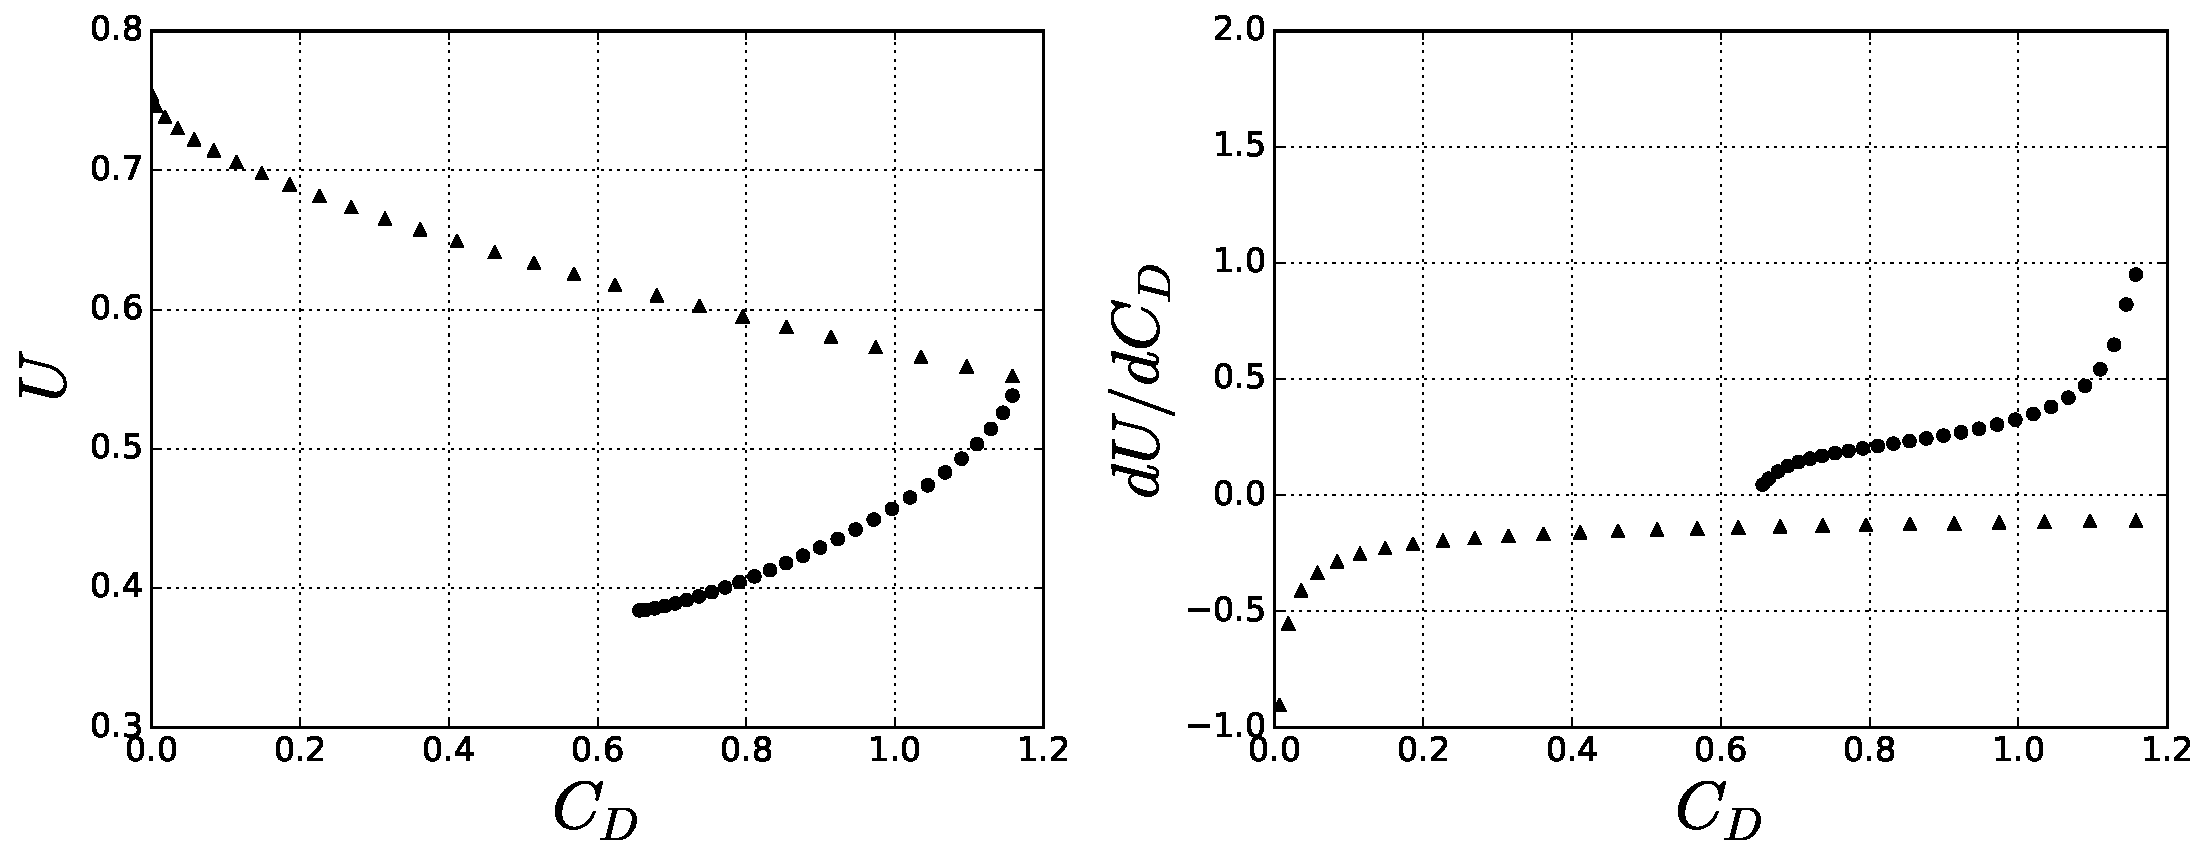
\includegraphics[width=1\linewidth]{chapter_3/figure/9}
	\caption{Case G. Left: mean velocity profile, $U$ , versus the drag coefficient, $C_d$ . Right: first derivative, $dU / d C_d$ . The triangles denote the region $y \in [0.76, 1]$, the filled circles denote the region $y \in [0.3, 0.76]$.}
	\label{fig:9}
\end{figure}

through their measurement data (cf. their Figure 7 and Equation (18)). We also notice that the deriv-
ative $dU/dC_d$ is reasonably small except locally at the point where the derivative of the function is
not continuous, where it is of order 1. The discontinuity there is however artificial since the function
$C_d(y)$ given in Equation (18) of \citet{ghisalberti2004limited}, where $C_d$ is divided into a parabolic and a
linear part, can be easily modified to yield a continuous first derivative at $y = 0.76$ if required, still
maintaining a mean flow very close to the measured one.

%%%%%%%%%%%%%%%%%%%%%%%%%%%%%%%%%%%%%%%%%%%%%%%%%%%%%%%%%%%%%%%%%%%%%%
\section*{Appendix B: a digression on spatial stability theory and group velocity}
%%%%%%%%%%%%%%%%%%%%%%%%%%%%%%%%%%%%%%%%%%%%%%%%%%%%%%%%%%%%%%%%%%%%%%

Stability problems such as the first one considered in this paper can be approached with the
spatial theory framework, with the wavenumber $\alpha$ complex, its imaginary part being a growth rate,
and the circular frequency $\omega$ a real constant parameter. Let us generalize the sensitivity analysis by
considering, as a first step, $\alpha$ and $\omega$ as complex numbers which can vary. Equation \ref{eq:lagid} contains one
additional term and reads:

\begin{equation}
0 = \delta \langle q^{\dagger}, \mathscr{L} q \rangle = 
\langle q^{\dagger}, \mathscr{L} \delta q \rangle +
\langle q^{\dagger}, \derp{\mathscr{L}}{U}  q \delta U\rangle +
\langle q^{\dagger}, \derp{\mathscr{L}}{C_d}  q \delta C_d\rangle +
\langle q^{\dagger}, \derp{\mathscr{L}}{\omega}  q \rangle \delta \omega +
\langle q^{\dagger}, \derp{\mathscr{L}}{\alpha}  q \rangle \delta \alpha
\label{eq:lagid_spatial}
\end{equation}

To obtain the sensitivities in the spatial problem (for which $\delta \omega = 0$) we now have to solve an adjoint
system similar to \ref{eq:uvp}, where $\omega^{\dagger}$ is replaced by $\omega$ and $\alpha$ by $\alpha^{\dagger}$ . The variation of the wavenumber  $\delta \alpha = 0$ is thus given by:

$$
\delta \alpha =\delta \alpha_r + i \delta \alpha_i= \int_0^{y_{\infty}}  G_U(y) \delta U(y) dy + \int_0^{1}  G_{C_D}(y) \delta C_D(y) dy
$$

the functions $G_U$ and $G_{C_d}$ maintain the same form as in the temporal theory \ref{eq:GCD}, with the direct and
adjoint eigenfunctions which are now normalized by imposing that $N_{\alpha} = -1$, with

$$
N_{\alpha} = \int_0^{y_{\infty}} \left[ \left(U - \dfrac{2i\alpha}{Re}\right) ( \overline{ v^{\dagger}} v +  \overline{ u^{\dagger}} u  )   +  \overline{ p^{\dagger}} u +  \overline{ u^{\dagger}} p  \right] d \; y
$$

Let us now consider a problem in which $U$ and $C_d$ are not allowed to vary, but $\alpha$ and $\omega$ are.
With reference to Equation \ref{eq:lagid_spatial}, with any choice of normalization of direct and adjoint modes, it
is found that $ N_{\omega} \delta \omega = N_{\alpha} \delta \alpha $. Thus, once the adjoint problem is solved, it is possible to accurately
compute the group velocity $c_g$ of any stability problem using the value of $ N_{\omega}$ and $ N_{\alpha}$ , i.e.,

\begin{equation}
c_g := \dfrac{d \omega_r}{d \alpha_r} \approx \dfrac{real(N_{\alpha})}{real(N_{\omega})}
\label{eq:group_vel}
\end{equation}

Note that $c_g$ above is different from the “complex group velocity” $C_g := \dfrac{d \omega}{d \alpha} \approx  \dfrac{N_{\alpha}}{N_{\omega}}$ , and it is also
$c_g \neq real(C_g)$. Relation \ref{eq:group_vel} can be employed in either a spatial or temporal stability analysis and
some representative results (for case G) are provided in Table I with the phase velocity $c_r := \omega_r / \alpha_r$
and the group velocity determined from Equation \ref{eq:group_vel} . The temporal or spatial amplification factors, $\omega_i$ or $-\alpha_i$ , respectively, are also given for all cases using Gaster’s transformation: $\omega_i = - \alpha_i c_g$ .
Two types of errors on the calculation of the group velocity (noted $err$) are given in the table; the top
four values, relative to the temporal theory, are defined as

$$
err = \dfrac{|c_g|_{\ref{eq:group_vel}} - c_g|_{FD}|}{c_g|_{\ref{eq:group_vel}}}
$$

with $c_g|_{FD}$ arising from a first-order finite difference approximation of the group velocity. The
bottom four values are defined by the formula

$$
err = \dfrac{|c_g|_{temporal} - c_g|_{spatial}|}{c_g|_{temporal}}
$$

The relative difference on $c_g$ between temporal and spatial theory is rather low. It has to be kept
in mind, however, that a stability analysis in the spatial framework yields a nonlinear eigenvalue
problem, with a consequent larger numerical system than in the temporal framework; therefore, by
inverting matrices of the same size, the accuracy is expected to be slightly lower. The accuracy of
the growth rate approximated through Gaster’s relationship is also found to be acceptable.

\begin{table}[H]
	\begin{center}
		\begin{tabular}{l|c|c|c|c|c|c|c|c}
			\hline 
			\hline
			Theory & $Re$ & $\alpha_r$ & $\omega_r$ & $-\alpha_i$ & $\omega_i$ & $c_r$ & $c_g$ & $err(\%)$ \\ 
			\hline 
			Temporal & 500 &\textbf{ 0.5}  & 0.4778 & \textit{0.0248} & 0.0254 & 0.9556 & 1.0245 & 0.54 \\ 
			
			& 3450 & \textbf{0.5}  & 0.4601 &\textit{ 0.0413} & 0.0404 & 0.9202 & 0.9797 & 0.06 \\ 
			
			& $10^5$ & \textbf{0.5 } & 0.4514 & \textit{0.0436} & 0.0421 & 0.9028 & 0.9661 & 0.63 \\ 
			
			& $10^9$ &\textbf{ 0.5}  & 0.4508 & \textit{0.0451} & 0.0425 & 0.9016 & 0.9427 & 2.90 \\ 
			
			Spatial & 500 & 0.4993 & \textbf{0.4778} & 0.0248 & 0.0250 & 0.9569 & 1.0100 & 1.41 \\ 
			
			& 3450 & 0.4990 & \textbf{0.4601} & 0.0427 & 0.0404 & 0.9220 & 0.9471  & 3.30 \\ 
			
			& $10^5$ & 0.4996 & \textbf{0.4514} & 0.0449 &  0.0416 & 0.9109 & 0.9371 & 3.46 \\ 
			
			& $10^9$ & 0.4993 & \textbf{0.4508} & 0.0450 & 0.0411 & 0.9028 & 0.9143 & 3.01 \\ 
			\hline 
			\hline
		\end{tabular} 
	\end{center}
	\label{tab:spa_tem}
	\caption{Temporal versus spatial stability, Case G. The model employed
		here is based on a modified Orr-Sommerfeld equation—rather than a system
		based on primitive variables as done in the bulk of the paper—which is
		why the temporal results have slightly larger growth rates $\omega_i$ than those
		displayed in Fig. \ref{fig:2}; this is related to the need of computing numerically
		$d^2 U /dy^2$ and $dC_d /dy$ in the Orr-Sommerfeld-like equation. In italics,
		the growth rates obtained from Gaster’s transformation are reported; the
		parameters imposed in each simulation are indicated with bold characters.
		The solutions for $Re = 10^9$ coincide with those found using the inviscid
		equations.}
\end{table}

The amplitude of the sensitivity functions, $|G_{U} ( y)|$ and $|G_{C_d} (y)|$, in the spatial and temporal
stability frameworks is of same order of magnitude (not shown here) since they are related through
temporal spatial the complex group velocity $C_g$ . It is found that $|{G_U}^{temporal}| \approx |C_g ||{G_U}^{spatial}|$ with $|C_g | \approx c_g \approx 1$ in the
present case.
Obtaining and comparing results in the temporal and spatial stability frameworks, such as in
Table I, is a good means to validate the sensitivity functions and to verify the accuracy of the
computations of the adjoint stability equations.


%%%%%%%%%%%%%%%%%%%%%%%%%%%%%%%%%%%%%%%%%%%%%%%%%%%%%%%%%%%%%%%%%%%%%%
\section*{Appendix C: comparison between continuous and discrete adjoint eigenfunctions}
%%%%%%%%%%%%%%%%%%%%%%%%%%%%%%%%%%%%%%%%%%%%%%%%%%%%%%%%%%%%%%%%%%%%%%

The discretization operation transform the operator $\mathcal{L}$ into a matrix $\mathbf{A}$ and of course do the same things to the unknown functions that becomes vectors.

\begin{table}[H]
	\begin{center}
		\begin{tabular}{|c|c|}
			\hline 
			continuous & discrete \\ 
			\hline 
			$\mathcal{L}$ & $\mathbf{A}$ \\ 
			\hline 
			$q$ & $\hat{q}$ \\ 
			\hline 
		\end{tabular} 
	\end{center}
\end{table}

This has a serious and most often hidden repercussion in th approach to solve the adjoint equations.

As above stated the derivation of the adjoint equation start with the enforcing of the Lagrange identity:

\begin{equation}
\langle q; \mathcal{L} q \rangle = \langle {\mathcal{L}}^{\dagger} q^{\dagger} ; q \rangle
\end{equation}

where the scalar product $ \langle ;\rangle$ is defined in our case as:

\begin{equation}
\langle a ; b\rangle = \int_{0}^{y_{\infty}} \overline{a} \cdot b dy \approx \sum_{i=1}^N \sum_{j=1}^N {\hat{\overline{a}}_i}^T w_{i,j} {\hat{b}_j} = {\hat{\overline{a}}_i}^T \mathbf{M} {\hat{b}_j} =  \langle a ; b\rangle_{\mathbf{M}}
\label{eq:scalr_prod}
\end{equation}

Is it clear from equation \ref{eq:scalr_prod} that the scalar product takes two different forms in the continuous and in the discrete case.
In fact in the discrete case is mandatory to introduce the quadrature rule weights $w_{i,j}$ of the chosen discretization.
$\mathcal{M}$ is the matrix representation of the weights and is symmetric and positive defined.

In order to compute and solve the adjoint equation one could proceed as follow:

\begin{itemize}
	\item The direct problem is defined in the continuous space as $\mathcal{L} q = 0$
	\item Chose a discretization (FEM, FD, Chebychev polynomials...) and transform the above problem in a discrete one $\mathbf{A} \hat{q}$
	\item Solve it to obtain the discrete version of the eigenfunctions $\hat{q}$
	\label{continuous}
\end{itemize}

For the adjoint problem on should at first compute the adjoint operator, this can be done using the Lagrangian identity at a continuous level:

\begin{equation}
\begin{split}
\langle q; \mathcal{L} q \rangle =& \langle {\mathcal{L}}^{\dagger} q^{\dagger} ; q \rangle \\
\Rightarrow \int_{0}^{y_{\infty}} \overline{q^{\dagger}} \; \mathcal{L} q  \; dy =& \int_{0}^{y_{\infty}} \overline{ {\mathcal{L}}^{\dagger} q^{\dagger}}  \; q  \; dy 
\end{split}
\end{equation}

From the last equation starting from the left part is it possible after some manipulation to retrieve the form on the right part and so find the formulation of the adjoint operator.

It is important to pinpoint that in the above equation the  scalar product $ \langle a ; b\rangle$ is enforced at a continuous level.

And now to solve the adjoint system the procedure \ref{continuous} can be used changing the direct system with the adjoint one.
The above way of computing the adjoint and solve the system is called \textbf{continuous approach}.

To summarize this approach one can straight forward solve th direct problem computationally, mathematically find the adjoint operator using the continuous scalar product and the Lagrange identity and then discretize the adjoint problem and solve it computationally.
This is why the \textbf{continuous approach} is sometimes known as derive than discretize.
And the stability and accuracy problems derive directly from the fact that we discretize the problem two times (the direct first and than the adjoint).


On the contrary in the \textbf{discrete approach} the scalar product \ref{eq:scalr_prod} is enforced at the discrete level in order to use the already discretized direct equation to retrive the adjoint system at a discrete level, to limit the computational errors.

\begin{equation}
\begin{split}
\langle q^{\dagger}; \mathcal{L} q \rangle =& \langle {\mathcal{L}}^{\dagger} q^{\dagger} ; q \rangle \\
\Rightarrow \overline{\hat{q}^{\dagger}}^T \mathbf{M} \mathbf{A} \hat{q}  =& \left( \overline{{\mathbf{A}}^{\dagger} \hat{q}^{\dagger}} \right)^{T} \mathbf{M} \hat{q} \\
\Rightarrow \mathbf{M} \mathbf{A}  =&  {\overline{\mathbf{A}^{\dagger}}}^T \mathbf{M} \\
\Rightarrow {\mathbf{A}}^{\dagger}  =&  \mathbf{M}^{-1} \mathbf{\overline{A}}^T \mathbf{M}
\end{split}
\end{equation}